
\documentclass[
	%parspace, % Add vertical space between paragraphs
	%noindent, % No indentation of first lines in each paragraph
	%nohyp, % No hyphenation of words
	%twoside, % Double sided format
	%draft, % Quicker draft compilation without rendering images
	%final, % Set final to hide todos
]{elteikthesis}[2024/10/26]

% The minted package is also supported for source highlighting
% See elteikthesis_minted.tex for example
%\usepackage[newfloat]{minted}
\usepackage{listings}
\usepackage{xcolor}
% Document's metadata
\title{Eventastic - Event Management System} % title
\date{2025} % year of defense

% Author's metadata
\author{Ali Afzal}
\degree{Computer Science BSc}

% Superivsor(s)' metadata
\supervisor{Gregory Morse} % internal supervisor's name
\affiliation{Lecturer} % internal supervisor's affiliation
%\extsupervisor{Jane Doe} % external supervisor's name
%\extaffiliation{Senior Developer} % external supervisor's affiliation

% University's metadata
\university{Eötvös Loránd University} % university's name
\faculty{Faculty of Informatics} % faculty's name
\department{Dept. of Programming Languages and Compilers} % department's name
\city{Budapest} % city
\logo{elte_cimer_szines} % logo

% Add bibliography file
\addbibresource{elteikthesis.bib}



% The document
\begin{document}

% Set document language
%\documentlang{hungarian}
\documentlang{english}

% List of todos (not in the final document)
%\listoftodos[\todolabel]

% Title page (mandatory)
\maketitle
% Topic declaration page (mandatory) - can also be attached instead
%\includepdf{topicdeclaration.pdf}

% Custom topic declaration page
\chapter*{Original Thesis Topic Declaration}


\begin{center}
   {\small
This thesis proposes the development of a comprehensive \textbf{Event Management System} designed to simplify the entire event lifecycle, from creation to execution. The system will feature a user-friendly interface allowing event organizers to efficiently set up and manage event details such as date, time, location, and attendee lists. It will also support robust user authentication and authorization to ensure secure access and data protection.

Key functionalities will include real-time notifications to keep users informed of any event updates or changes, and advanced search and filtering options to help users find events based on specific criteria like location and date. The system will facilitate attendee management through features like RSVP capabilities and attendee tracking, enhancing both security and engagement.

Additionally, the system will integrate analytics and reporting tools to provide organizers with insights into event popularity, attendee demographics, and engagement metrics. This will aid in making informed decisions to optimize future events. Overall, the thesis focuses on delivering a scalable, efficient solution that enhances event organization, improves attendee experience, and provides actionable insights through data analysis.

\vspace{0.5em} % Adjust vertical spacing

\noindent \textbf{Features:}
\begin{enumerate}
    \item \textbf{Event Creation and Management:} Users can create events, set details like date, time, location, and manage attendees.
    \item \textbf{User Authentication and Authorization:} Implement secure user management with roles for event creators, attendees, and administrators.
    \item \textbf{Real-time Notifications:} Notify users about updates like new events, changes, or reminders.
    \item \textbf{Search and Filtering:} Search for events based on location, date, or category.
    \item \textbf{Event Participation:} RSVP to events, and event creators can manage attendees.
    \item \textbf{Analytics and Reporting:} Insights into event popularity, attendee demographics, and engagement.
\end{enumerate}
}
\end{center}

\vfill % Pushes the content to the center vertically

\cleardoublepage

% Table of contents (mandatory)
\tableofcontents
\cleardoublepage

% Main content
\chapter{Introduction}
\label{ch:intro}

The organization of successful events, encompassing personal, corporate, or social contexts, necessitates careful planning and effective oversight of various details. Nonetheless, this process frequently becomes unwieldy owing to the presence of disjointed tools and manual coordination activities. This thesis advocates for the creation of a novel \textbf{Event Management System} designed to enhance and facilitate the event planning process.

The suggested system aims to encompass the complete lifecycle of events, ranging from their inception to their execution, while tackling significant obstacles encountered by both event organizers and participants. Through the provision of an intuitive interface, this system will facilitate event creators in the seamless management of critical information such as dates, venues, and participant lists. Furthermore, robust authentication procedures and role-based access controls will safeguard data integrity and guarantee suitable user permissions.

The principal characteristics of the system encompass real-time notifications designed to keep users updated, sophisticated search and filtering options to locate pertinent events, and RSVP functionalities for monitoring participation. Furthermore, the incorporation of analytics and reporting instruments will equip organizers with actionable insights, including attendee demographics and engagement metrics, thus promoting data-driven decision-making.

This thesis examines the development of a scalable, efficient, and accessible web-based solution designed to enhance event management and simultaneously elevate the user experience. The primary objective is to convert event planning into a smooth and engaging experience for both organizers and participants.
\cleardoublepage

\chapter{User documentation}
\label{ch:user}

This chapter serves as a user guide to help readers navigate the platform and utilize its features efficiently. By the end of this chapter, users will understand how to create and manage events, interact with the platform as different roles (organizers and attendees), and perform critical actions such as submitting RSVPs, uploading files, and processing payments.

The application is built using Next.js\cite{nextjs} with React\cite{react} for the frontend, leveraging TypeScript\cite{typescript} for type safety and Tailwind CSS\cite{tailwindcss} for responsive and accessible design. The backend utilizes MongoDB\cite{mongodb} as the database, managed through Mongoose\cite{mongoose}, with server-side functionality powered by Next.js API routes. Authentication is handled through Clerk\cite{clerk}, which provides secure session management, role-based access, and OAuth integration. File uploads are managed using Uploadthing\cite{uploadthing}, and payments are integrated with Stripe\cite{stripe} for secure and scalable transaction processing.

Due to the absence of a registered business entity, the application is only available for local deployment, and payment functionalities are demonstrated through mock transactions. While the current setup is sufficient for demonstration purposes, future iterations can include online hosting and live payment processing to make the platform fully operational for real-world use cases.


\section{User Role and Capabilities}
In \textbf{Eventastic}, every user account is designed to support a wide range of capabilities, enabling users to seamlessly act as both event attendees and organizers. This approach simplifies the user experience by allowing a single account to handle all actions related to discovering, participating in, and hosting events.

\subsection{General User Actions}
All users in the system can:
\begin{itemize}
    \item Search for events based on location, date, category, or keywords.
    \item View detailed information about events, including date, time, venue, and ticket options.
    \item Purchase tickets to events or RSVP for free events.
    \item Manage their profile and view a list of registered or upcoming events.
\end{itemize}

\subsection{Event Hosting Capabilities}
In addition to attendee functionalities, users can also create and manage events, effectively acting as organizers. These capabilities include:
\begin{itemize}
    \item Creating and publishing events by filling out forms with event titles, descriptions, locations, dates, ticket pricing, and images.
    \item Managing ticket sales, tracking RSVPs, and viewing attendee details in real-time.
    \item Editing event details or canceling events when necessary.
    \item Sending notifications or updates to registered attendees.
    \item Accessing analytics and insights to evaluate event performance, such as ticket sales, attendance trends, and other metrics.
\end{itemize}

\subsection{Unified User Experience}
Since every account supports both attendee and organizer functionalities, there is no need for separate accounts. Users can seamlessly switch between discovering events to attend and managing events they organize. This unified design ensures that users have all the tools they need to participate in or host events without additional complexity.

\textit{Note:} The terms \textbf{User}, \textbf{Attendee}, and \textbf{Organizer} are used interchangeably throughout this documentation, as they all refer to a single account type with extended capabilities based on user actions.






\section{Software Requirements and How to Start the
Program}

To host the website locally, the user must have \textbf{Node.js}\cite{nodejs} installed
in advance. This software is a popular runtime JavaScript environment, used to run
the JavaScript\cite{javascript} projects of any kind. Along with Node.js, the installation will also set
up \textbf{Node Package Manager (npm)}\cite{npm}. By using this package
manager, the user can add, remove or update packages necessary for the project.
The official installation guide can be found at \textit{https://nodejs.org/en/learn/getting-started/how-to-install-nodejs}

After installation, one can verify by following these steps.

\begin{itemize}
	\item Open a terminal or a command prompt depending on your operating system.
	\item Type \textit{node -v} and \textit{npm -v} and press Enter. This Figure~\ref{fig:terminal-1} shows a successful
installation of Node.js program. The versions of the software can be seen as a
result.
\end{itemize}



\begin{figure}[H]
	\centering
	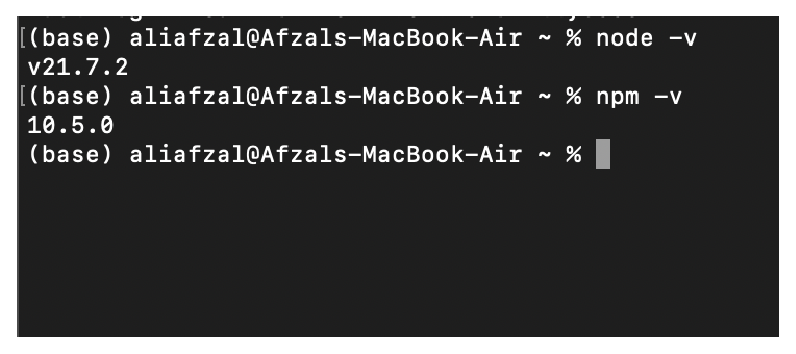
\includegraphics[width=0.6\textwidth,height=100px,frame]{images/terminal1.eps}
	\caption{How to Verify Node.js Installation}
        \label{fig:terminal-1}
\end{figure}


Run the following command from the root directory in order to  install the dependencies :

\lstset{caption={Install Packages Command}}
\begin{lstlisting}
npm install
\end{lstlisting}


The next step involves setting up environment variables, create a new file named \textit{.env} in the root of your project and add the following content:
\lstset{caption={.env file contents}}
\begin{lstlisting}
#NEXT
NEXT_PUBLIC_SERVER_URL=

#CLERK
NEXT_PUBLIC_CLERK_PUBLISHABLE_KEY=
CLERK_SECRET_KEY=
NEXT_CLERK_WEBHOOK_SECRET=

NEXT_PUBLIC_CLERK_SIGN_IN_URL=/sign-in
NEXT_PUBLIC_CLERK_SIGN_UP_URL=/sign-up
NEXT_PUBLIC_CLERK_AFTER_SIGN_IN_URL=/
NEXT_PUBLIC_CLERK_AFTER_SIGN_UP_URL=/

#MONGODB
MONGODB_URI=

#UPLOADTHING
UPLOADTHING_SECRET=
UPLOADTHING_APP_ID=

#STRIPE
STRIPE_SECRET_KEY=
STRIPE_WEBHOOK_SECRET=
NEXT_PUBLIC_STRIPE_PUBLISHABLE_KEY=
\end{lstlisting}

Replace the placeholder values with your actual credentials.

Next, run the following command and open \textit{http://localhost:3000} in your browser to view the project.
\lstset{caption={Install Packages Command}}
\begin{lstlisting}
npm run dev
\end{lstlisting}


\section{Features}

This part of the documentation entails the features of our website. The readers
will understand the usage of each web component after this section.


\subsection{Common Features}

The common features are the ones which appear in most of the pages. They
include components like header, navigation bar, profile menu and footer. See Figure~\ref{fig:header}

\begin{figure}[H]
	\centering
	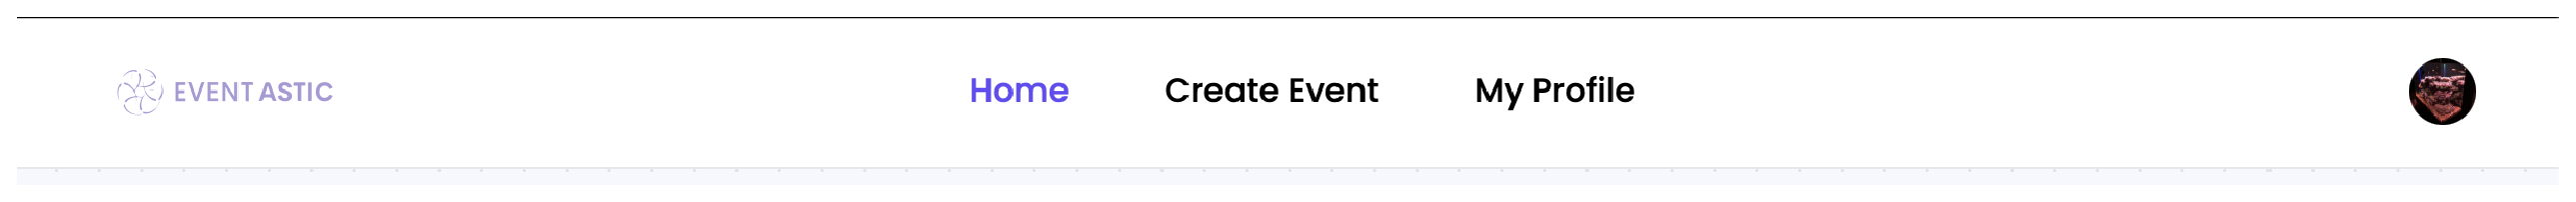
\includegraphics[width=1.0\textwidth,height=40px,frame]{images/header.eps}
	\caption{Header and Navigation Bar}
        \label{fig:header}
\end{figure}



Profile menu can be activated by clicking on the user icon in the navigation
bar. Figure~\ref{fig:profile} shows a list of account related menu for the user.

\begin{figure}[H]
	\centering
	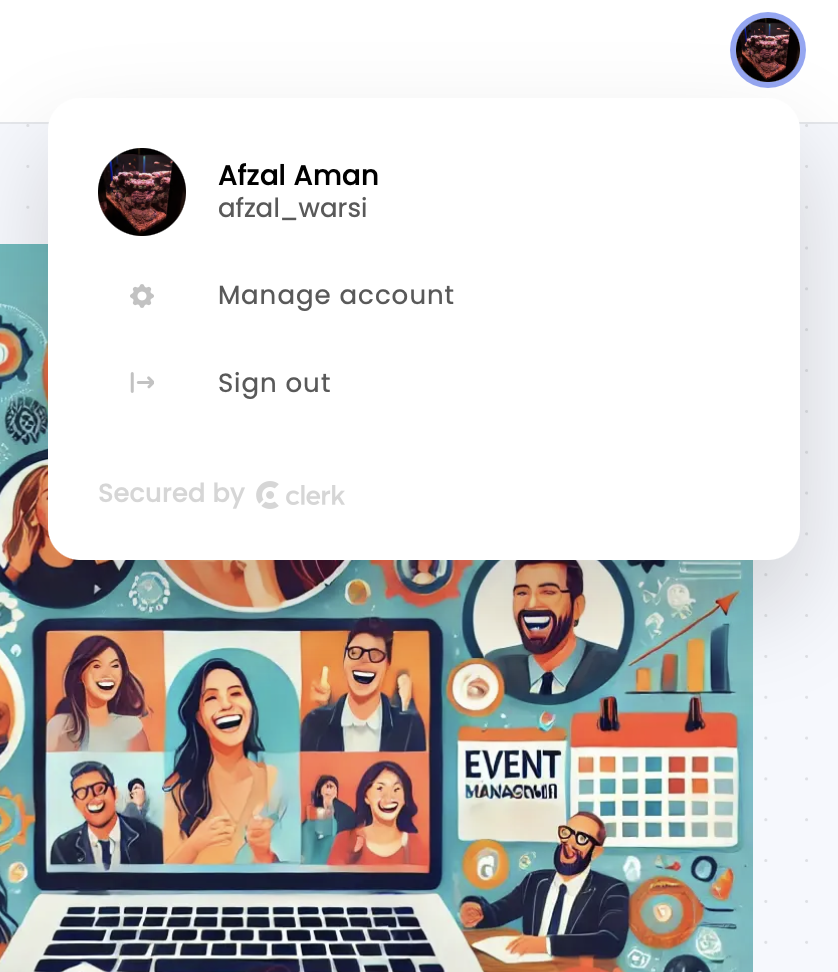
\includegraphics[width=0.6\textwidth,height=250px,frame]{images/profile.png}
	\caption{Profile Menu}
        \label{fig:profile}
\end{figure}

From this menu, the users can register, log in or log out from their accounts, or
manage their profiles.

\begin{figure}[H]
	\centering
	
\includegraphics[width=1.0\textwidth,height=40px,frame]{images/footer.png}
	\caption{footer}
        \label{fig:footer}
\end{figure}

\subsection{Registration}

The Register link in the profile menu will redirect the user to the Register page.
The user must fill out the form and complete the process by clicking the register
button. The user can also choose to register via \textbf{Google}. The information needed is as shown in Figure~\ref{fig:register}

\begin{figure}[H]
	\centering	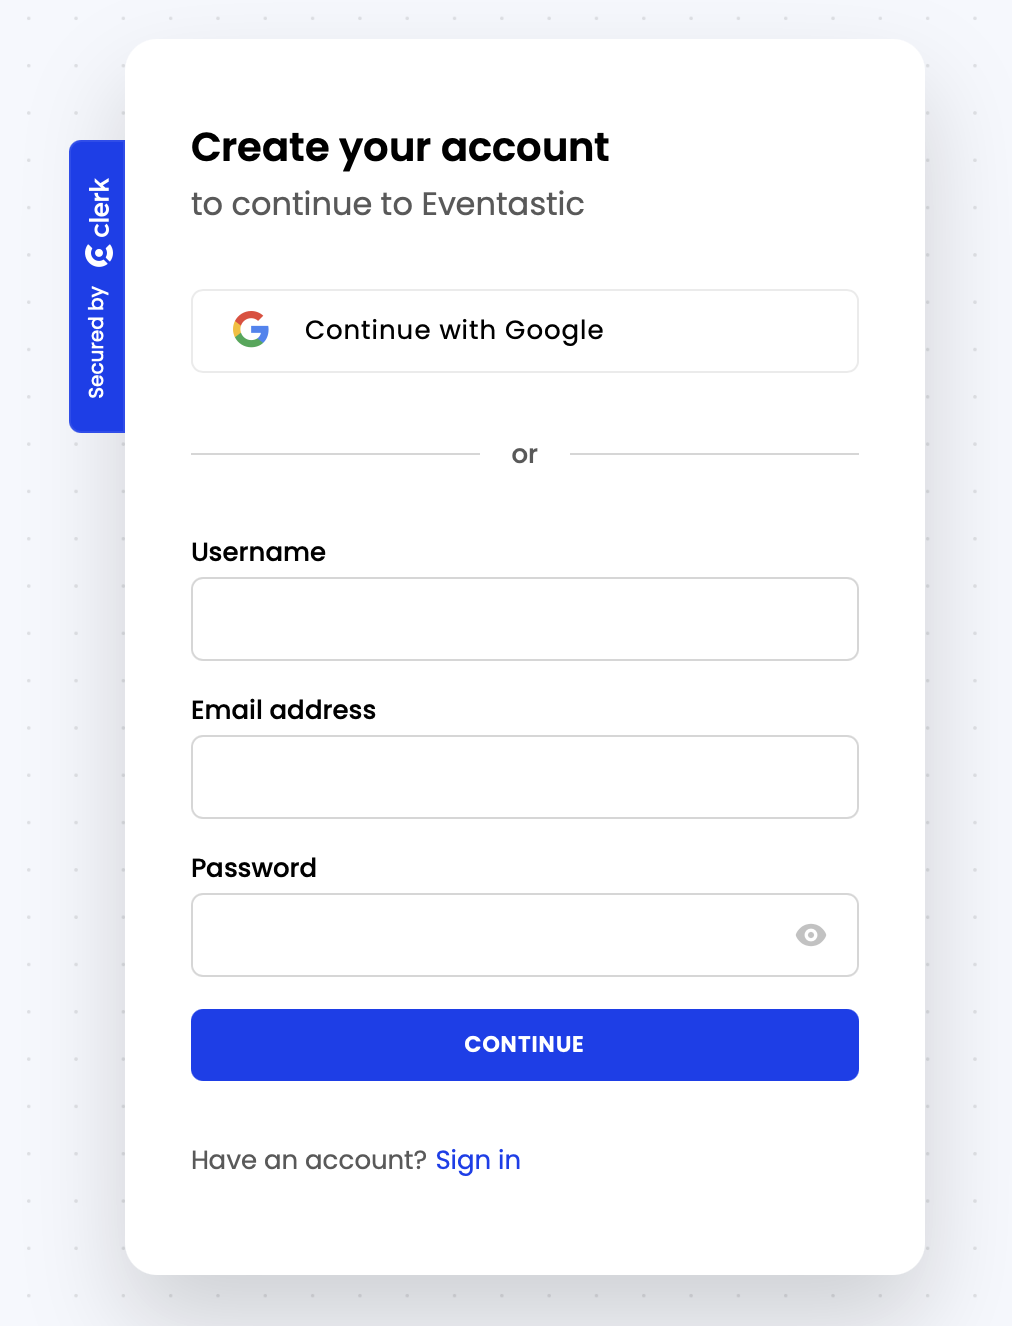
\includegraphics[width=0.6\textwidth,height=300px,frame]{images/register.png}
	\caption{User Registration Form}
        \label{fig:register}
\end{figure}


\subsection{Logging In}


After a successful registration, users will be taken to the login page. They can
either log in there or manually by activating the profile menu and using the link
there instead, see Figure~\ref{fig:login}. Once clicked on \textit{continue}, the user will be prompted to enter the password.

\begin{figure}[H]
	\centering	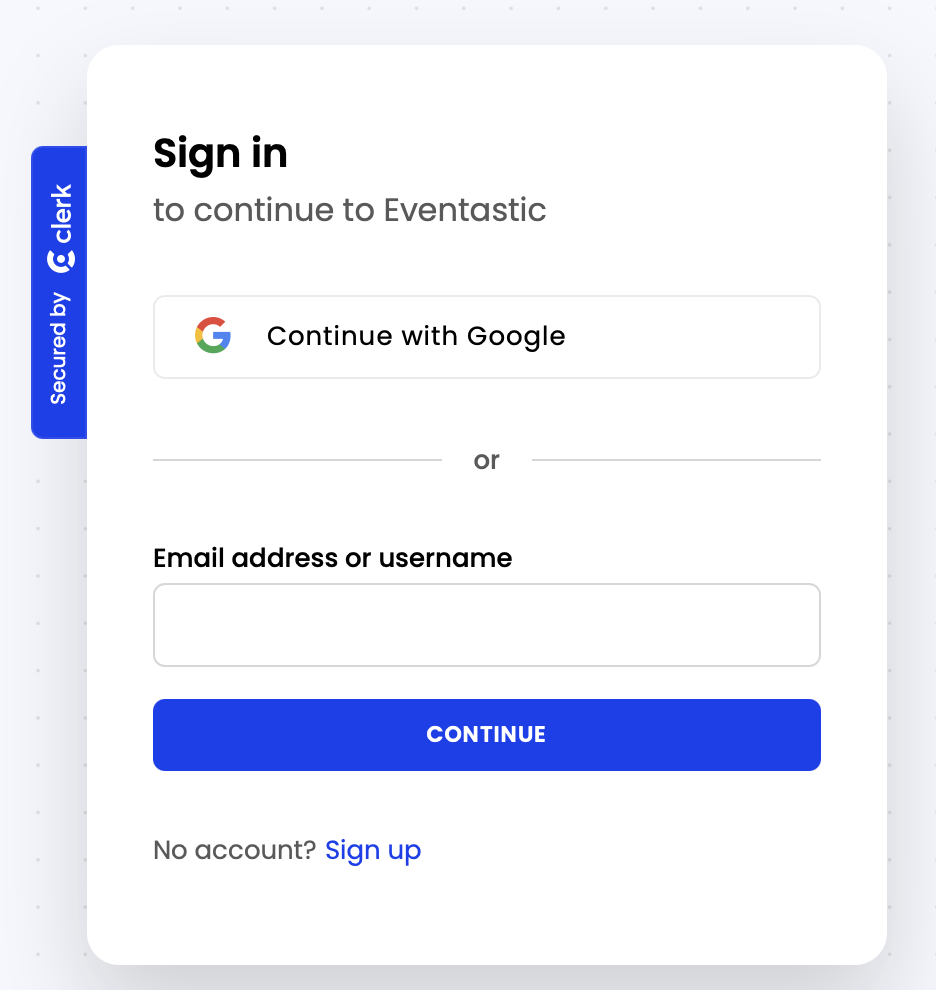
\includegraphics[width=0.6\textwidth,height=300px,frame]{images/login.png}
	\caption{User Registration Form}
        \label{fig:login}
\end{figure}


\subsection{My Profile}
The \textbf{My Profile} page in \textbf{Eventastic} serves as a central hub for users to manage both their purchased tickets and the events they organize. This section provides an overview of the key functionalities available on the profile page see Figure~\ref{fig:profile1} below.

\begin{figure}[H]
	\centering	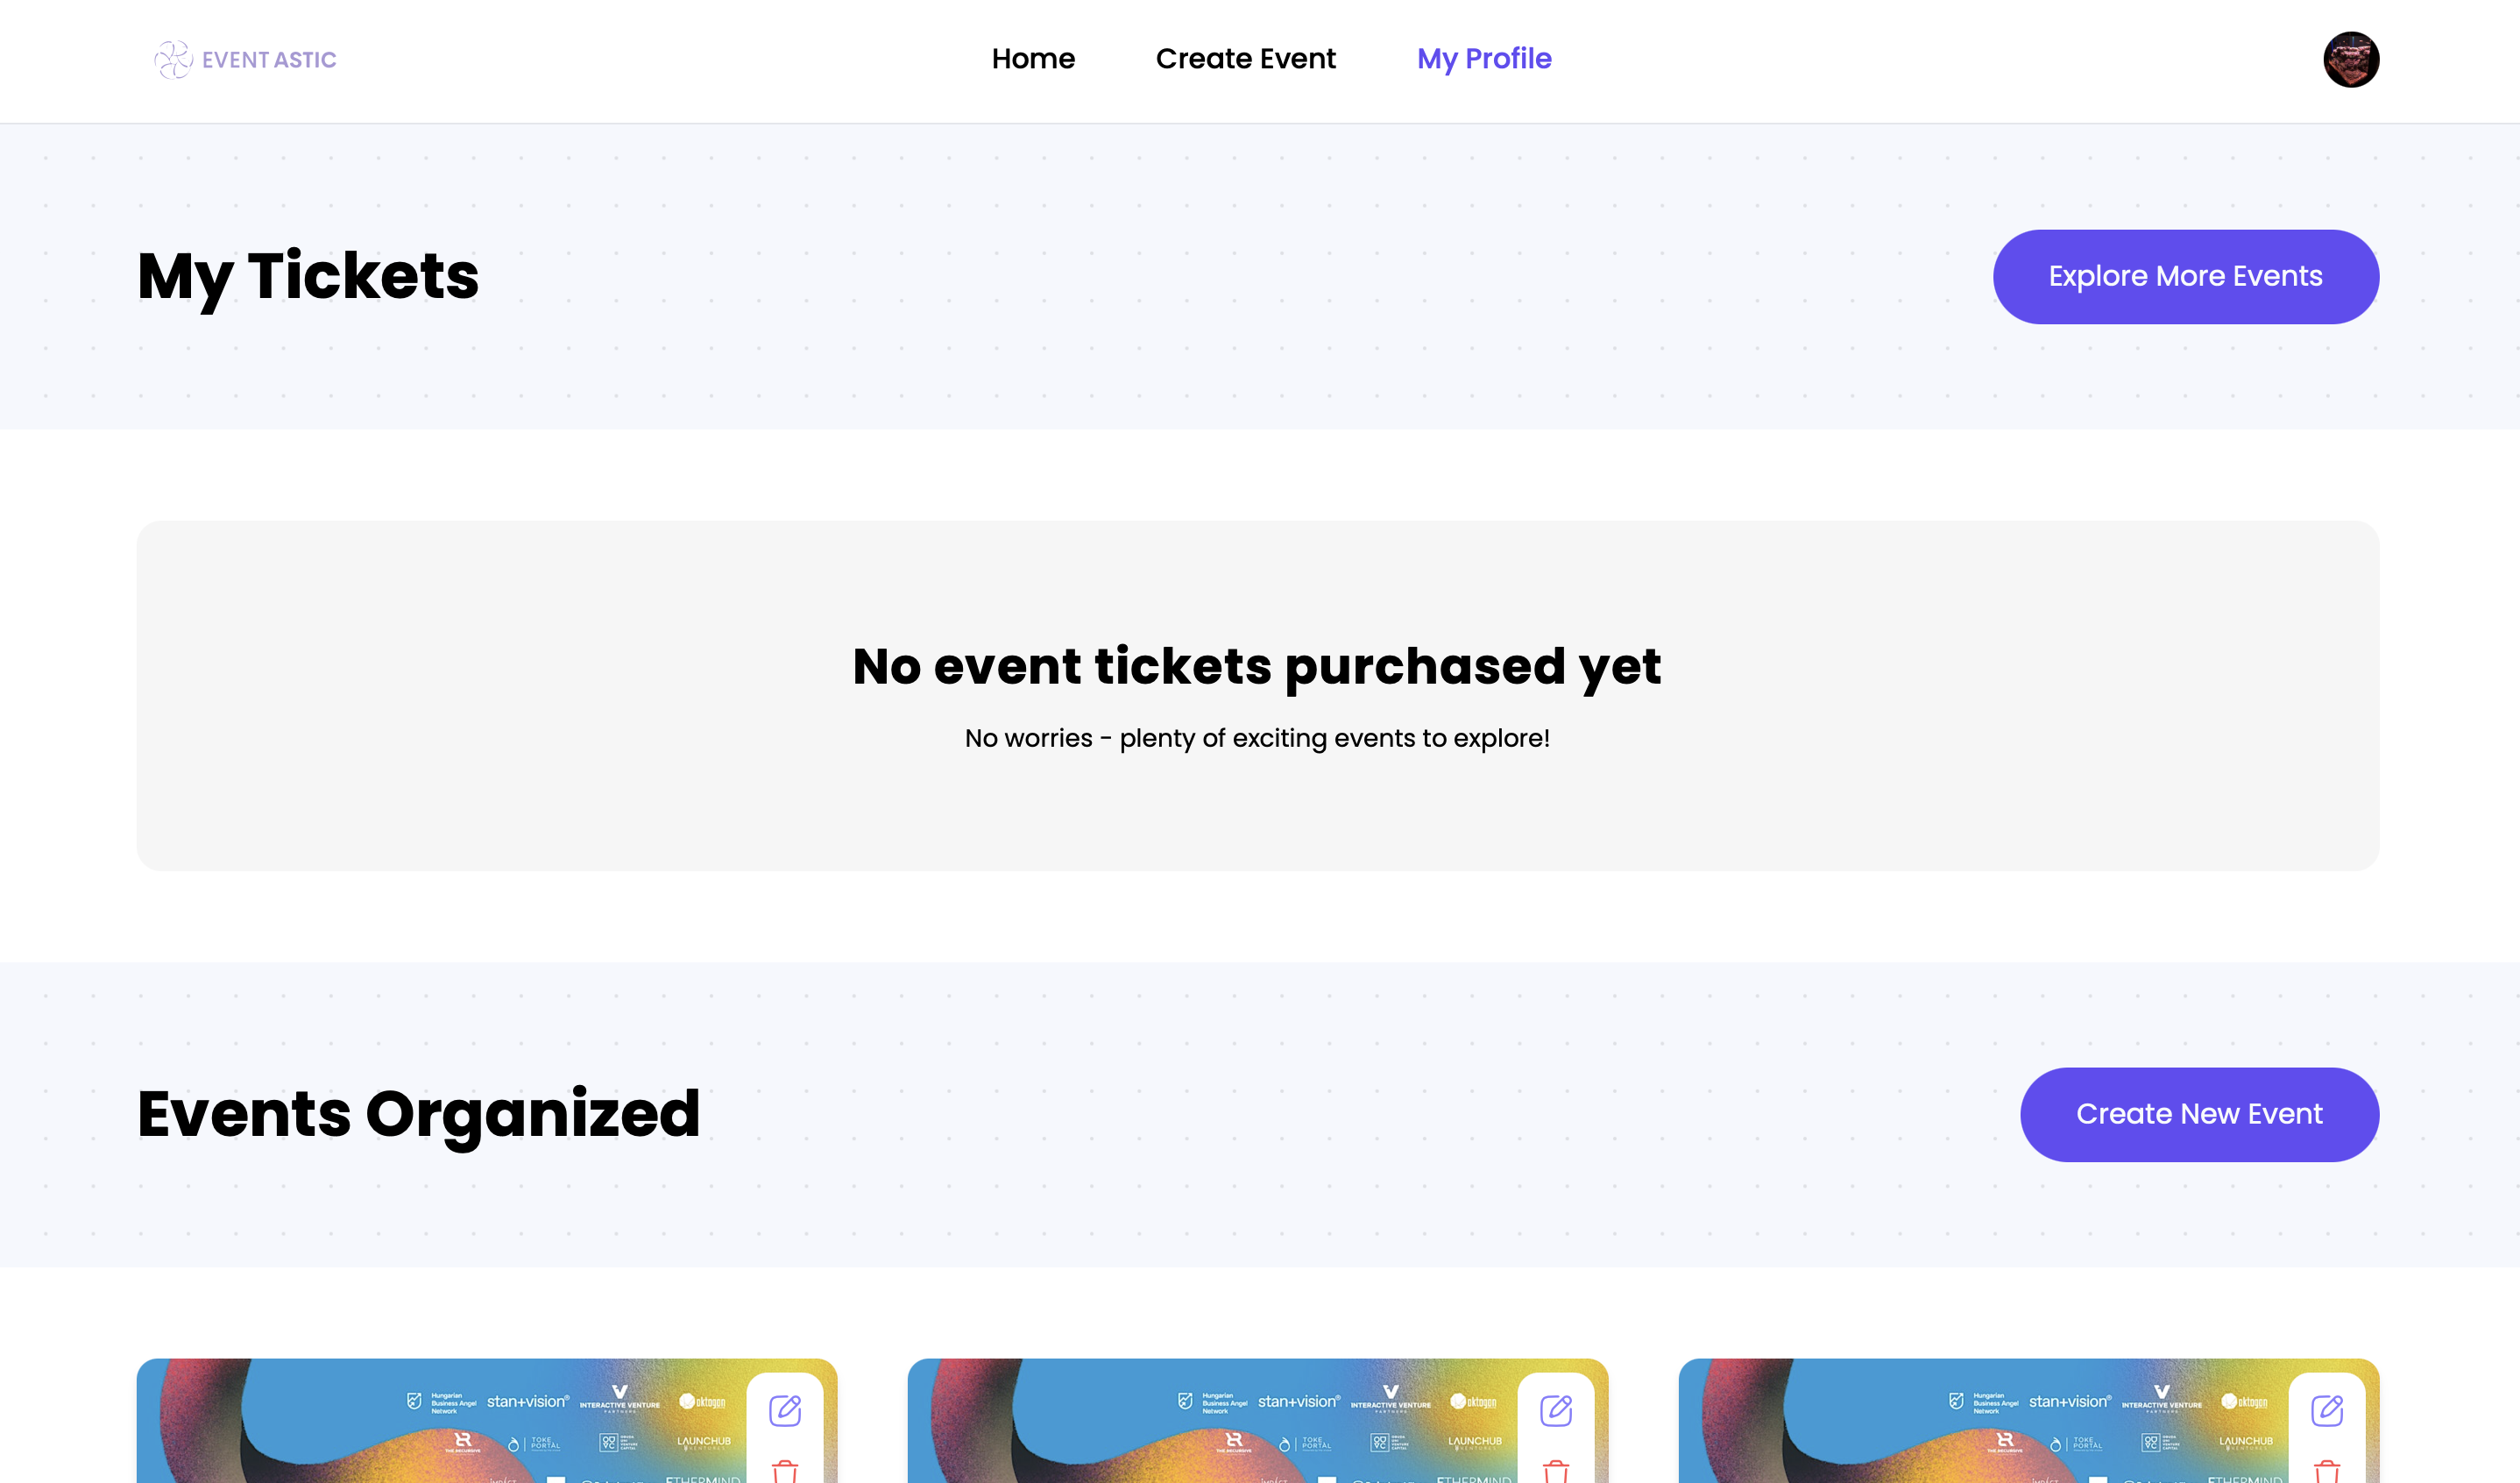
\includegraphics[width=1.0\textwidth,height=300px,frame]{images/profile1.png}
	\caption{My Profile Page 1}
        \label{fig:profile1}
\end{figure}

The \textbf{My Tickets} section displays a comprehensive list of all events for which the user has either purchased tickets or submitted an RSVP. Each event in this list is clickable, allowing users to navigate directly to the corresponding event page. On the event page, users can view detailed information about the event, including the date, time, location, and other relevant details.

\begin{figure}[H]
	\centering	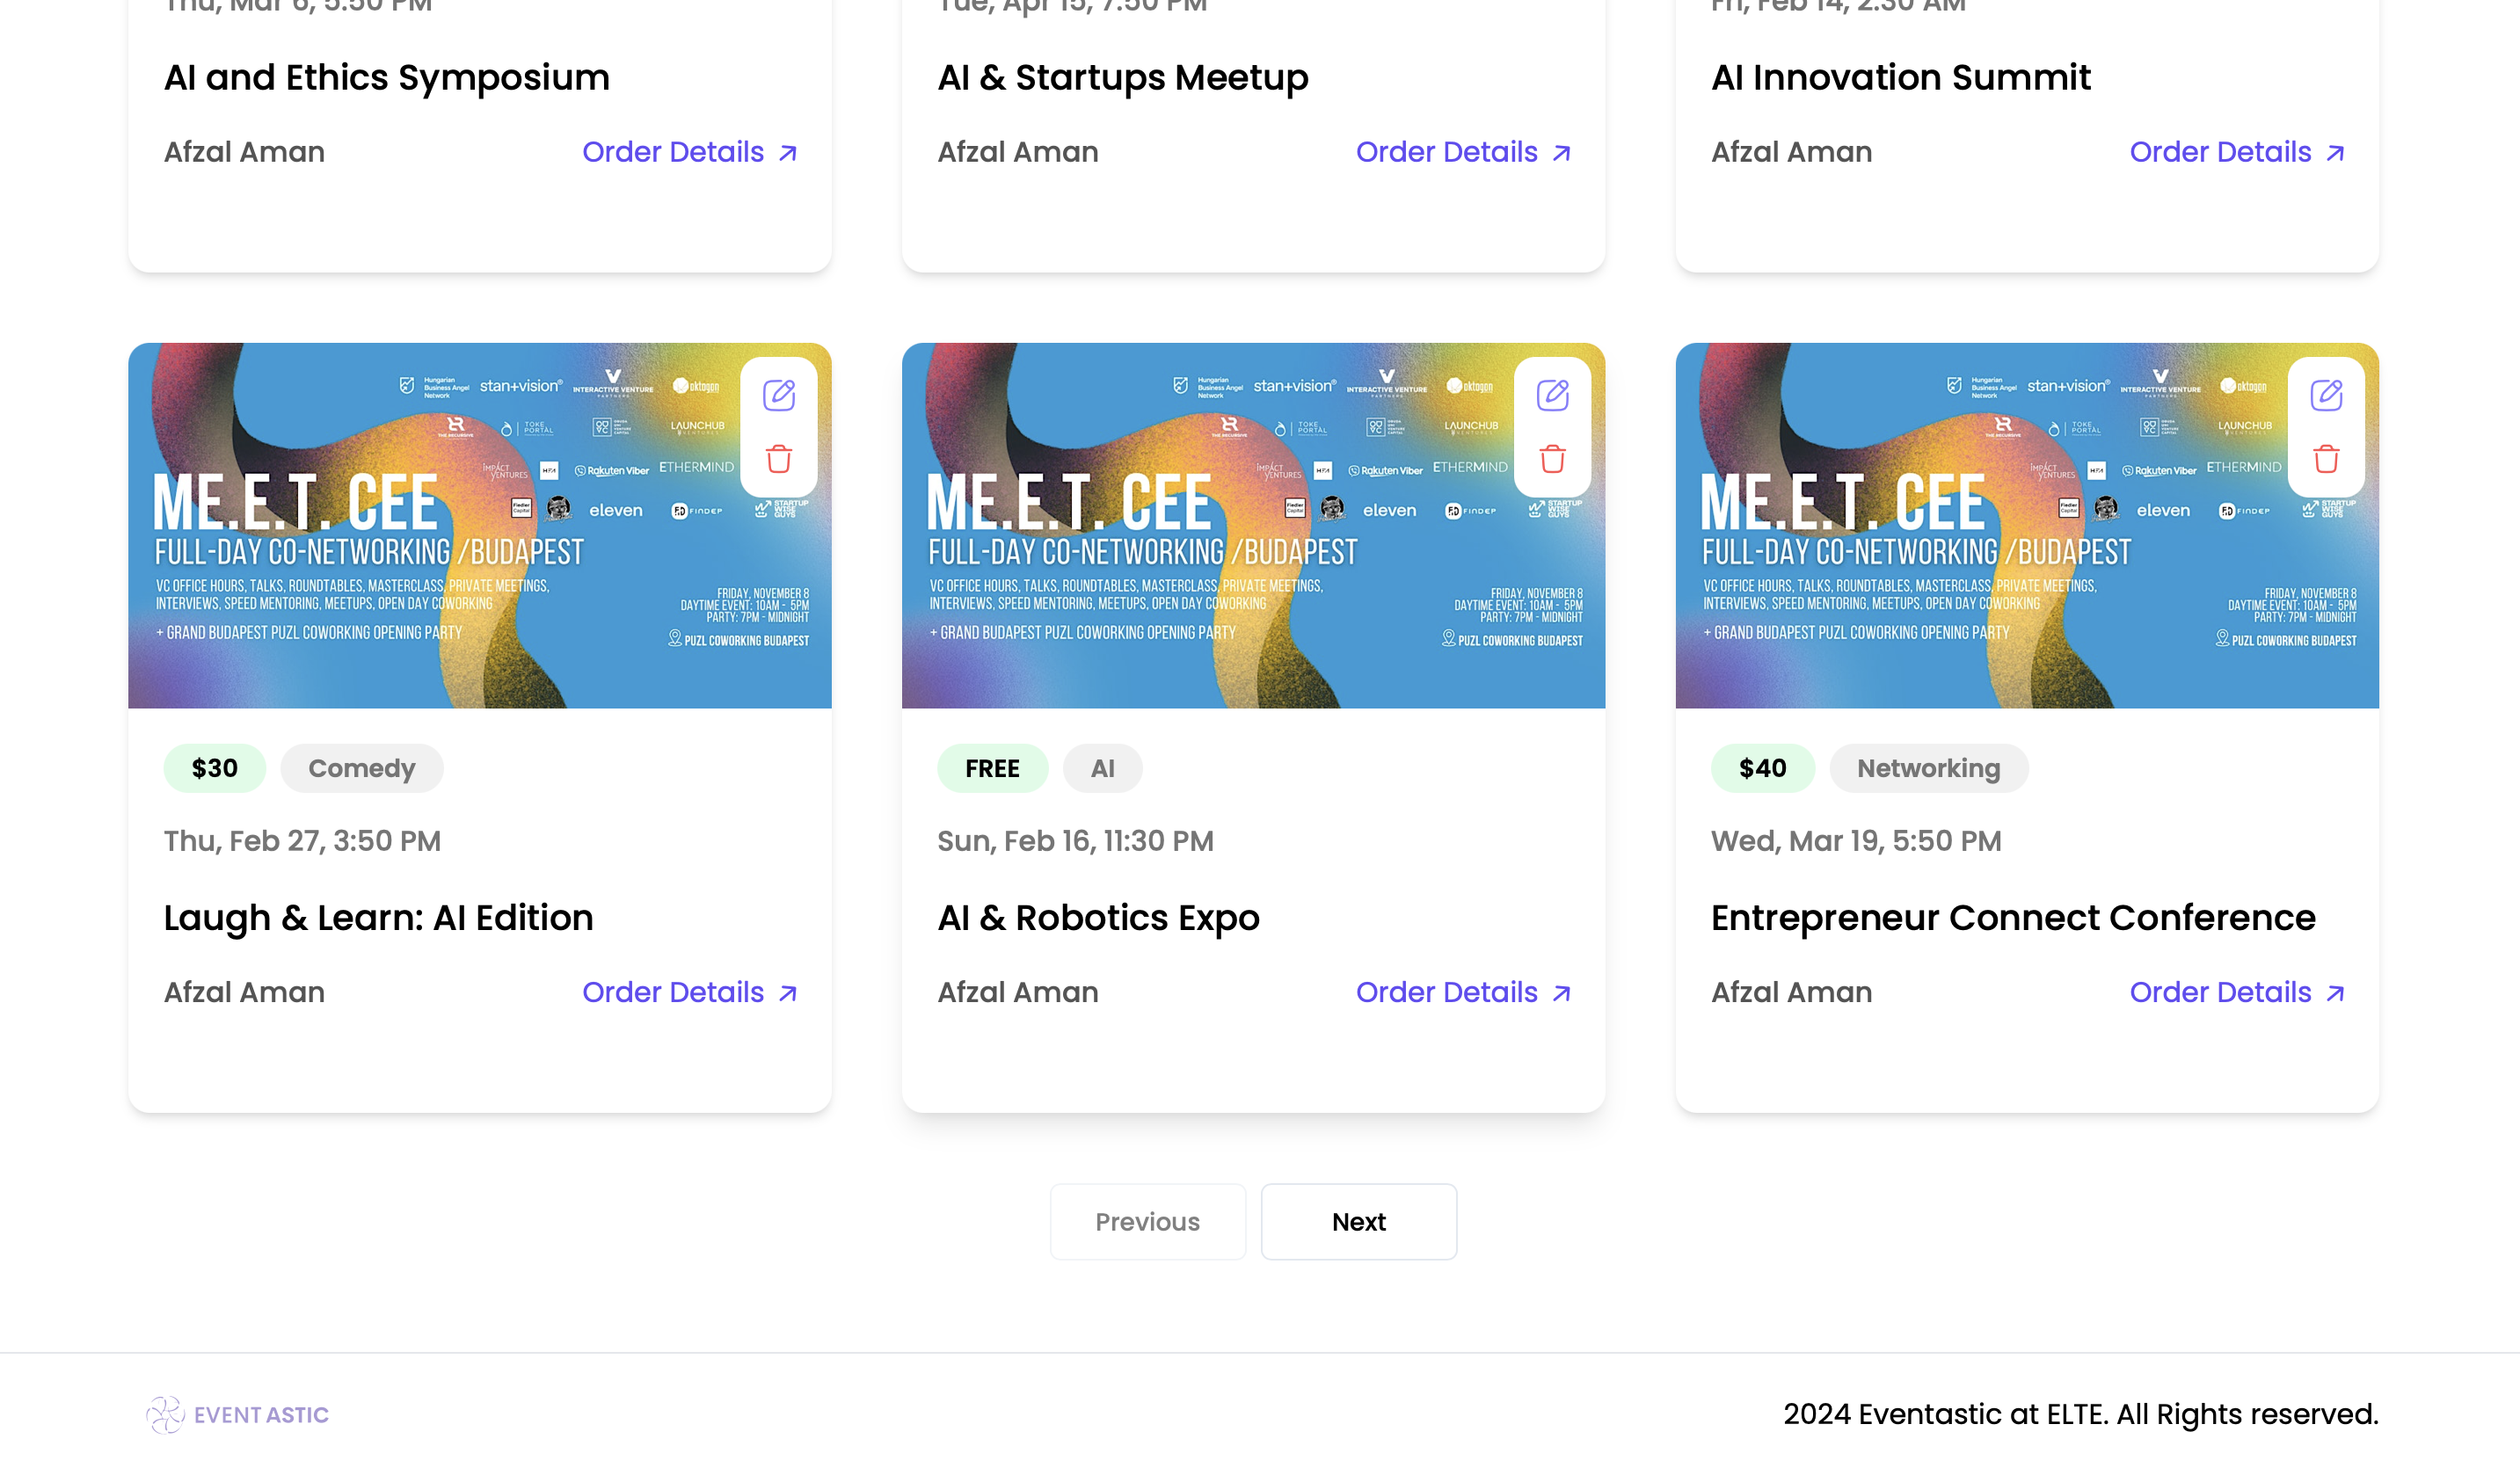
\includegraphics[width=1.0\textwidth,height=300px,frame]{images/profile2.png}
	\caption{My Profile Page 2}
        \label{fig:profile2}
\end{figure}


The \textbf{Events Organized} section (see Figure~\ref{fig:profile2}) provides users with a list of all the events they have created. For each event in this list, the following options are available:
\begin{itemize}
    \item \textbf{Edit Event:} Allows users to modify the event details such as title, description, date, time, location, ticket pricing, or other event-specific information.
    \item \textbf{Delete Event:} Enables users to permanently remove an event from the platform if it is no longer needed.
    \item \textbf{Order Details:} This button provides users with an overview of all the attendees and order details associated with the event. This feature is particularly useful for organizers to track ticket sales, RSVPs, and attendee information efficiently.
\end{itemize}

\textbf{My Profile} ensures that users can manage their interactions with the platform, whether they are attending events or organizing them, all from a single, intuitive interface.



\subsection{Event Search and Filtering}

\begin{figure}[H]
	\centering	
\includegraphics[width=1.0\textwidth,height=80px,frame]{images/search1.png}
	\caption{Search filter}
        \label{fig:search1}
\end{figure}

\textbf{Eventastic} provides an intuitive and efficient event search functionality to help users quickly find events of interest. 

Users can search for events by simply entering the event name in the search bar see Figure~\ref{fig:search1} above. The search process is dynamic and happens in real time, displaying matching results as the user types. This ensures a seamless and responsive experience, allowing users to locate specific events effortlessly.

To enhance the search functionality, a filtering system is implemented. Users can refine their search results by specifying the \textbf{category} of the event. This feature enables a more targeted search, ensuring that users can easily discover events that match their preferences and interests.


\begin{figure}[H]
	\centering	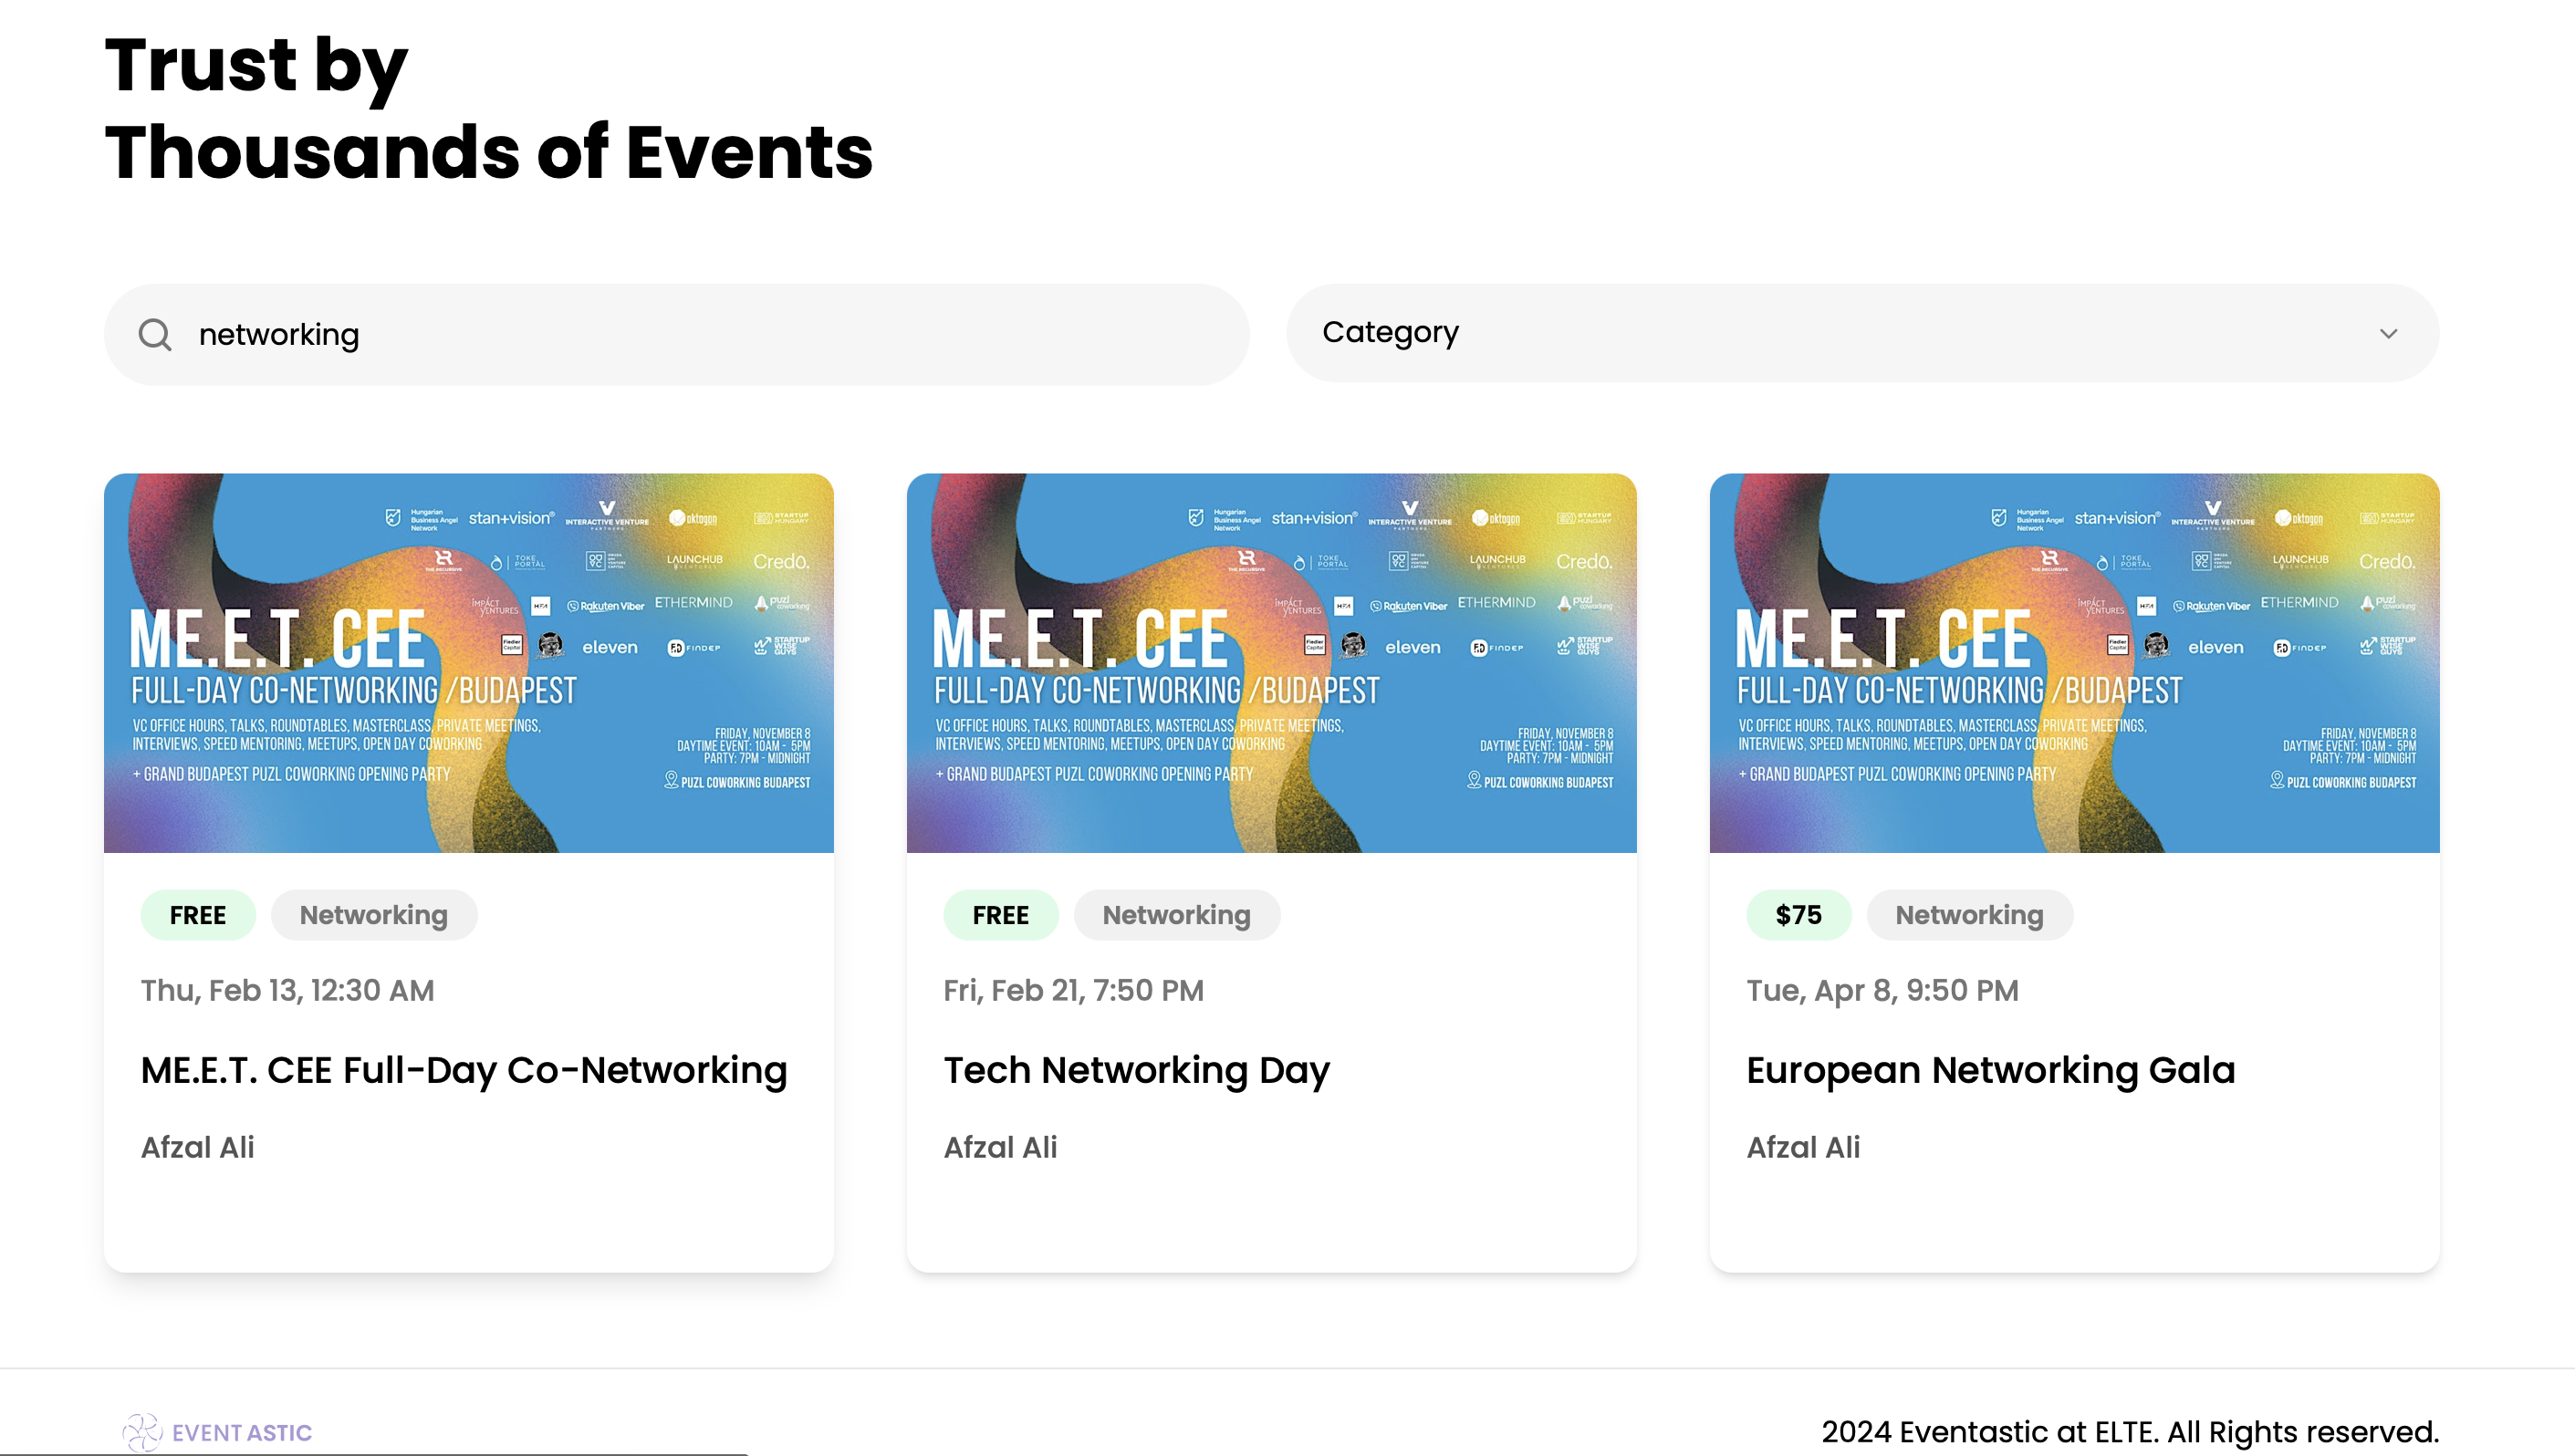
\includegraphics[width=1.0\textwidth,height=300px,frame]{images/search2.png}
	\caption{Search Event Result}
        \label{fig:search2}
\end{figure}


The combination of real-time search and category filtering ensures a user-friendly and efficient event discovery process, catering to the diverse needs of the platform’s users.


\subsection{Event Page}

The \textbf{Event Page} in \textbf{Eventastic} provides users with comprehensive details about each event. It is designed to deliver all essential information at a glance, ensuring users can make informed decisions about their participation. 

The event page displays all relevant details about the event, including:
\begin{itemize}
    \item \textbf{Cost:} Ticket pricing or indication if the event is free.
    \item \textbf{Category:} The type of event (e.g., music, workshop, seminar).
    \item \textbf{Organizer Details:} Information about the event organizer.
    \item \textbf{Location:} Venue or online meeting link for the event.
    \item \textbf{Start and End Date/Time:} Precise timing of the event.
    \item \textbf{Description:} A detailed description providing an overview of the event.
    \item \textbf{External Links:} Additional resources or references for the event.
\end{itemize}

\begin{figure}[H]
	\centering	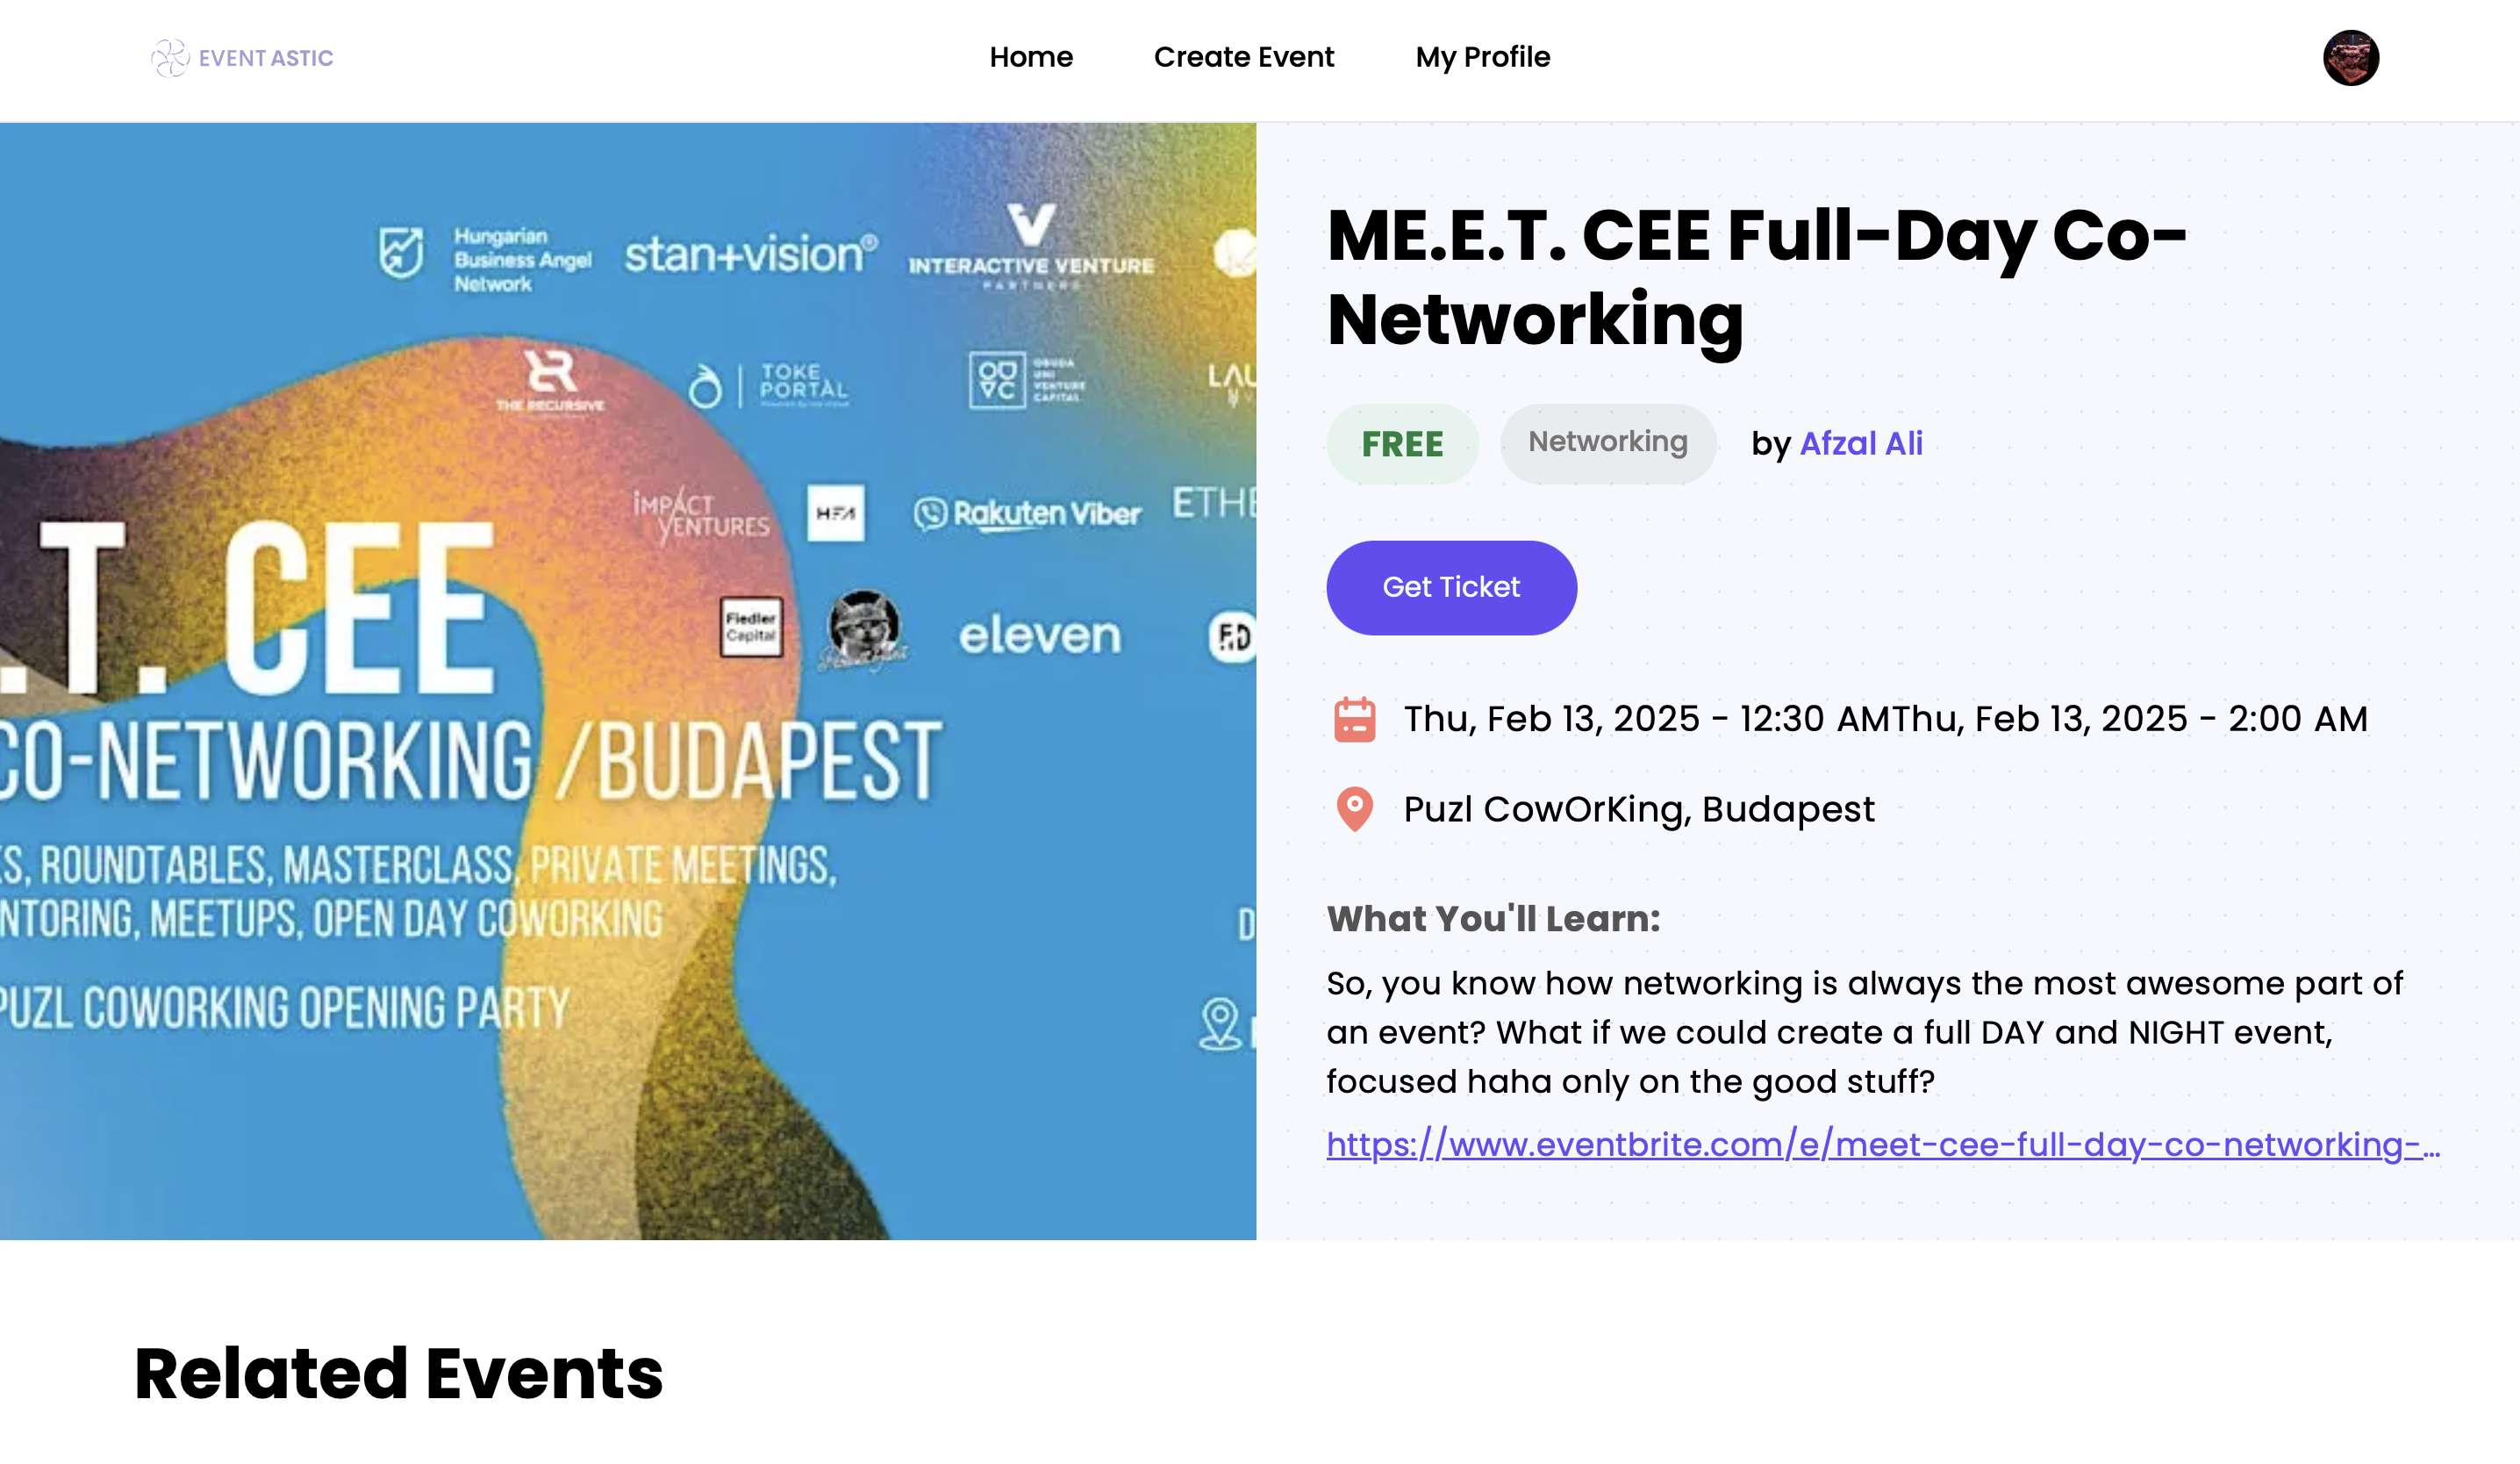
\includegraphics[width=1.0\textwidth,height=300px,frame]{images/event.png}
	\caption{Event Page}
        \label{fig:event}
\end{figure}

The page includes a prominent \textbf{"Get Ticket"} button, allowing users to seamlessly purchase tickets or RSVP for the event directly from the page.

At the bottom of the event page, users can discover \textbf{Related Events}, which are recommendations based on similar categories or user preferences. This feature enhances event discovery and encourages further engagement on the platform.

The event page is designed to provide a rich and user-friendly experience, presenting all critical information in a structured and visually appealing manner.


\subsection{Checkout Process}
The \textbf{Checkout Process} in \textbf{Eventastic} is streamlined to provide users with a seamless experience when purchasing event tickets. 

When a user wishes to purchase a ticket for an event, they can click the \textbf{Buy Ticket} button available on the event page. This action redirects the user to the \textbf{Stripe Payment Gateway} see Figure~\ref{fig:checkout} below , where the transaction is processed.


\begin{figure}[H]
	\centering	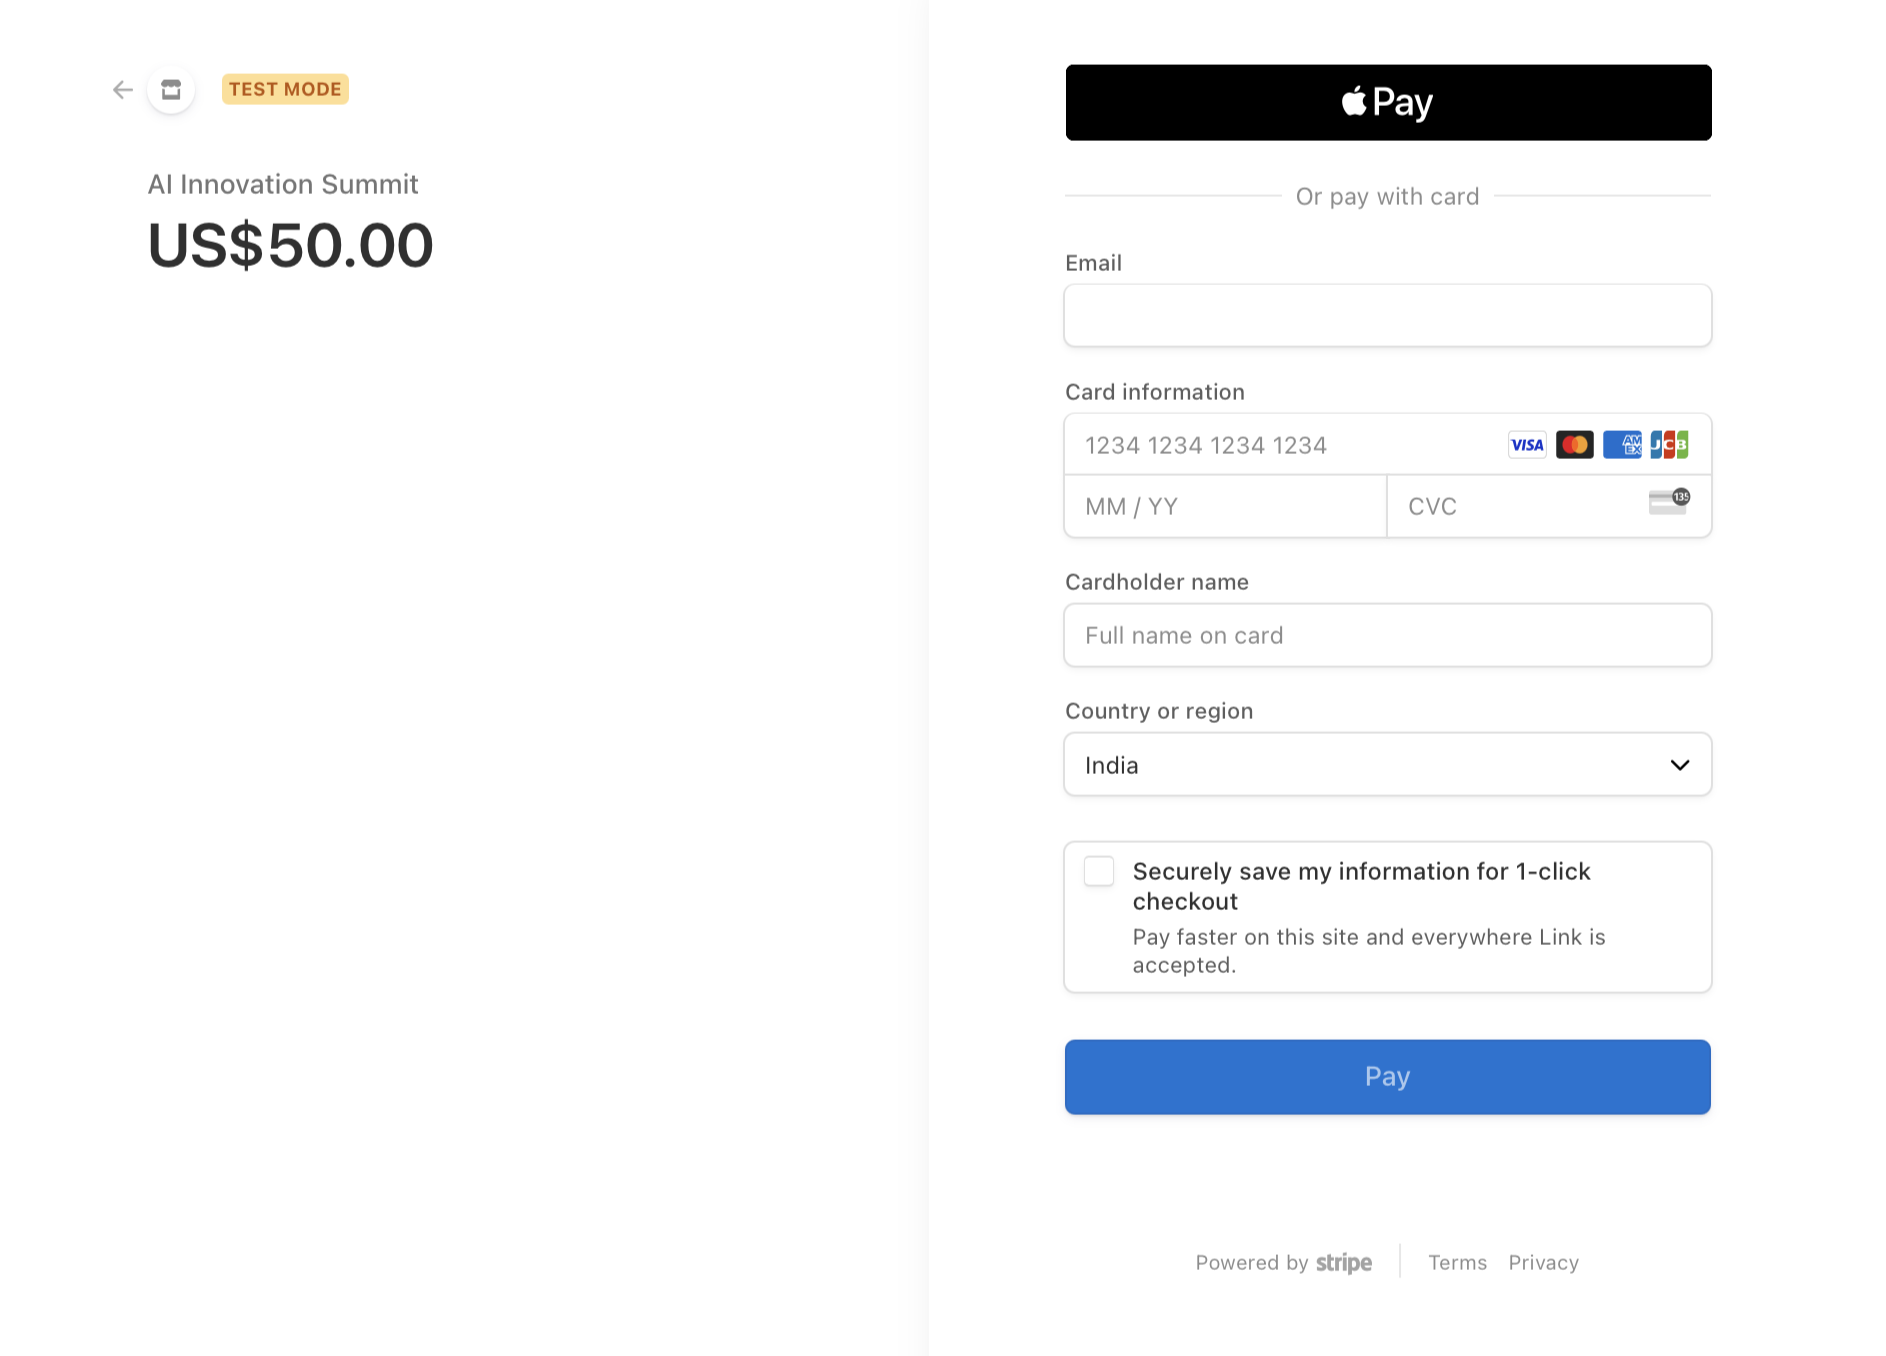
\includegraphics[width=1.0\textwidth,height=300px,frame]{images/checkout.png}
	\caption{Checkout Page}
        \label{fig:checkout}
\end{figure}

Since the platform operates in \textbf{test mode}, users are required to follow the \textbf{test payment routine} to simulate transactions. Stripe provides a variety of test card credentials for this purpose. Users can refer to the official \href{https://stripe.com/docs/testing}{Stripe Documentation} for a comprehensive list of test card options. 

For example, using the card number \texttt{4242 4242 4242 4242} with any valid expiration date and CVV will simulate a successful transaction.

There is also an option for \textbf{Apple Pay} or \textbf{Google Pay} depending on the user's operating system.

Upon completing the payment, the user is automatically redirected back to the platform. The result of the transaction is displayed on the confirmation page:
\begin{itemize}
    \item For \textbf{successful payments}, a confirmation message is shown, indicating that the ticket purchase was successful.
    \item For \textbf{failed payments}, an error message is displayed, informing the user of the issue.
\end{itemize}

This process ensures a user-friendly and secure payment experience while enabling developers and testers to simulate real-world scenarios effectively.


\subsection{Creating an Event}
The \textbf{Create Event} feature allows users to host and publish their events on the \textbf{Eventastic} platform seamlessly.

To create an event, the user can simply click on the \textbf{Create Event} button located in the navigation bar. This action opens a comprehensive event creation form.


The event creation form requires the user to input essential details about the event, including:
\begin{itemize}
    \item \textbf{Event Title:} A descriptive title for the event.
    \item \textbf{Description:} Detailed information about the event.
    \item \textbf{Location:} The venue or link for the event.
    \item \textbf{Start and End Dates/Times:} The schedule for the event.
    \item \textbf{Ticket Price:} Cost of tickets (or mark the event as free).
    \item \textbf{External Links:} Optional links, such as additional resources or social media.
    \item \textbf{Category:} Choose an appropriate category from the existing list or add a new one if needed.
\end{itemize}

If the user wishes to create a new event category beyond the available options, the form provides an easy-to-use \textbf{Add Category} feature see Figure~\ref{fig:createEvent2} below. This ensures flexibility in categorizing events appropriately.

Once all the required details are filled out, the user can click the \textbf{Create Event} button at the bottom of the form. This action instantly makes the event live on the platform, allowing it to be viewed and accessed by other users.

The event creation page is designed for simplicity and efficiency, ensuring users can create events quickly while providing all necessary details. A visual example of the form is shown in Figure~\ref{fig:createEvent1}.

\begin{figure}[H]
	\centering	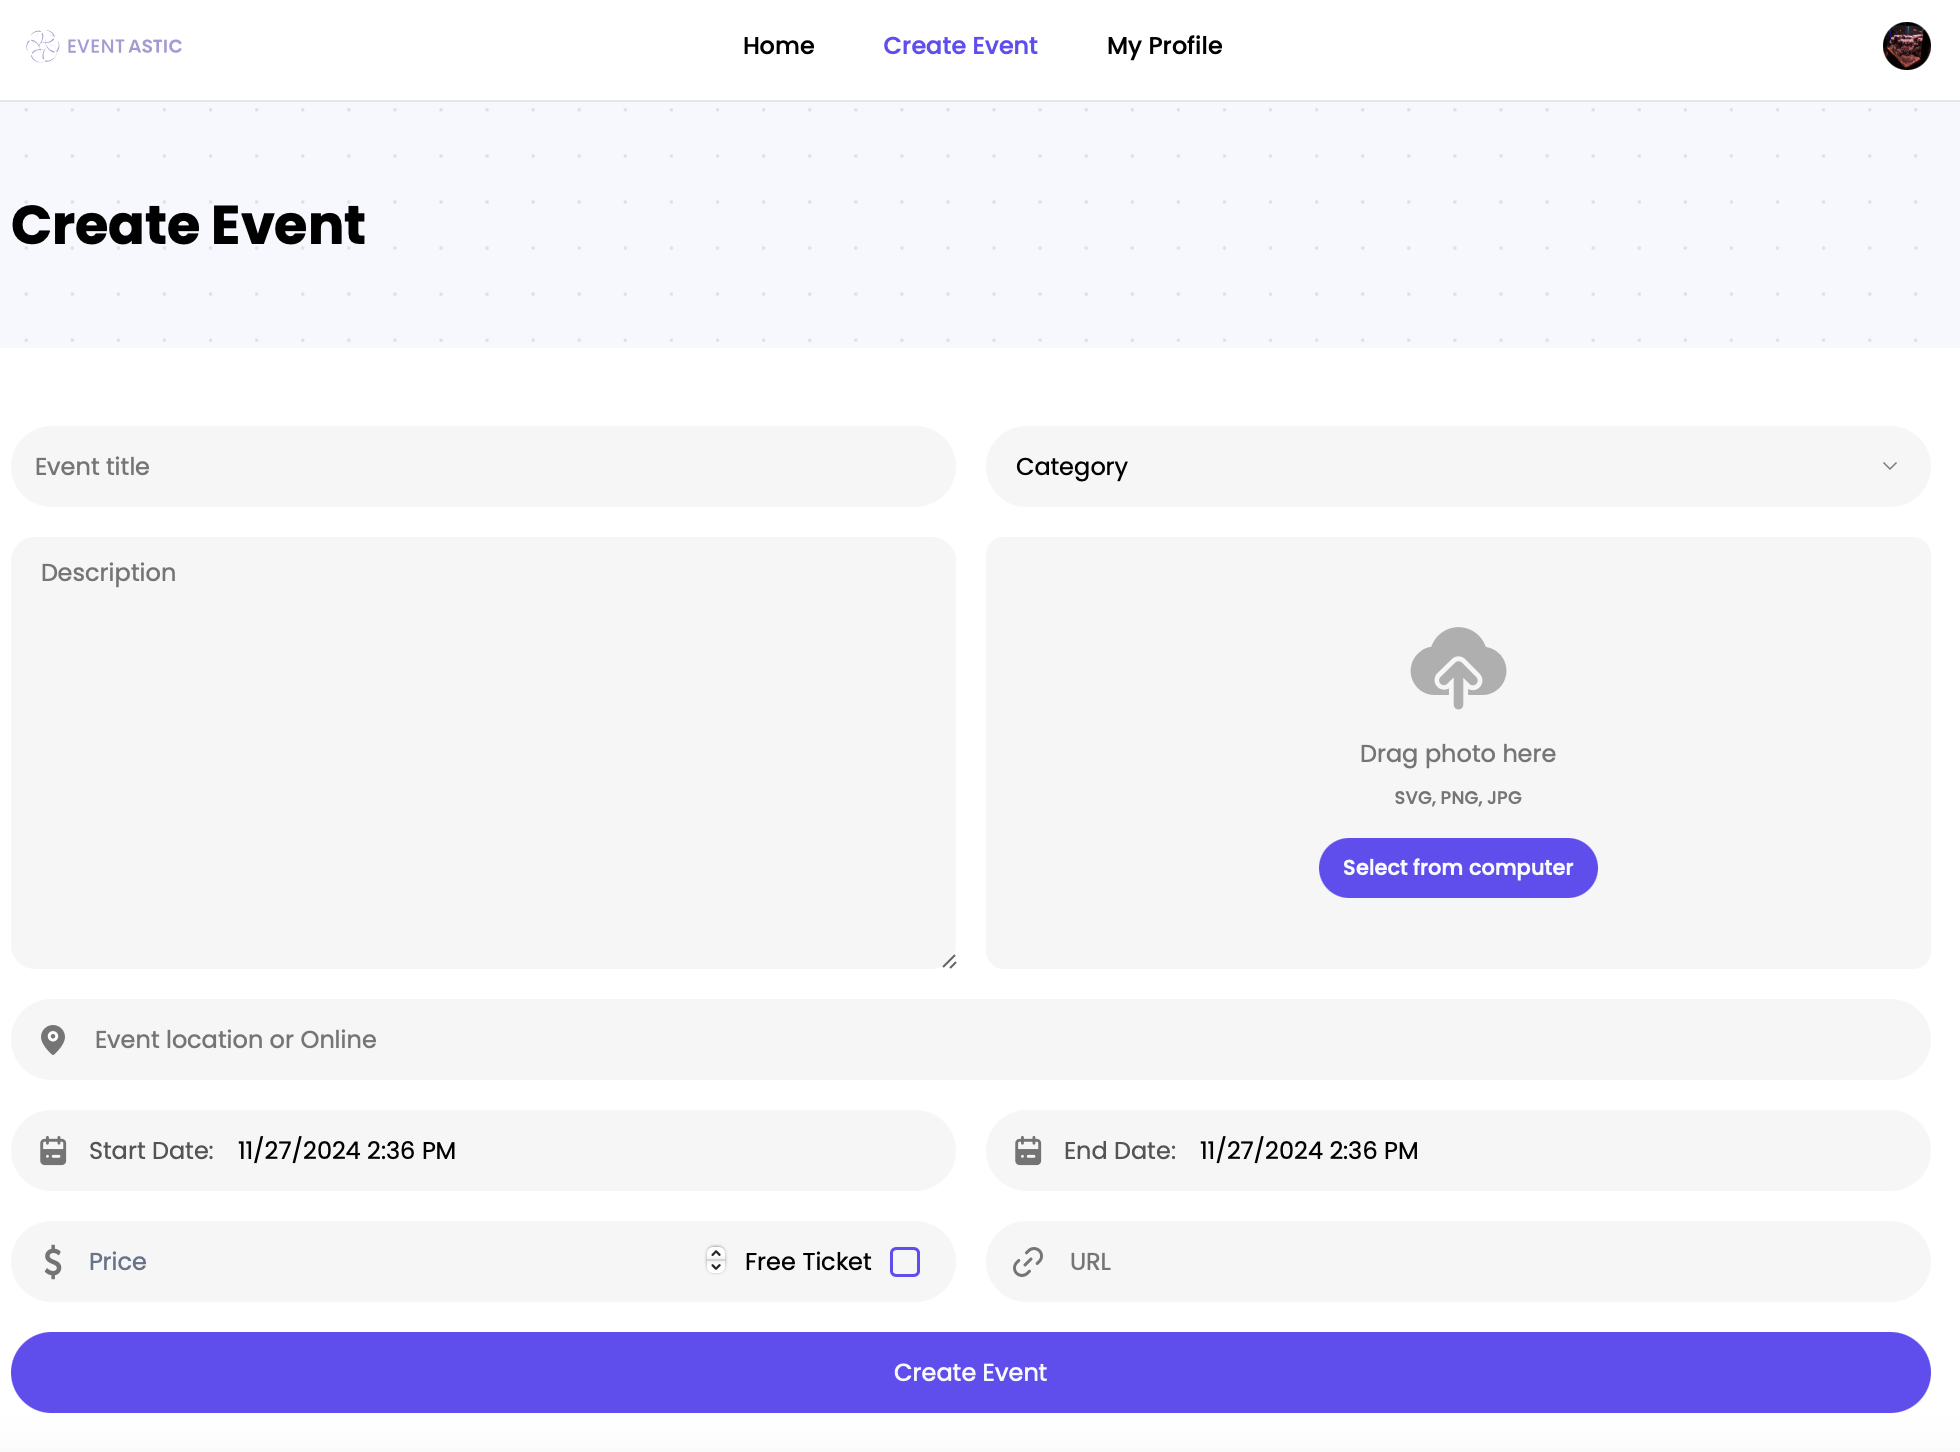
\includegraphics[width=1.0\textwidth,height=300px,frame]{images/createEvent1.png}
	\caption{Create Event Page}
        \label{fig:createEvent1}
\end{figure}


\begin{figure}[H]
	\centering	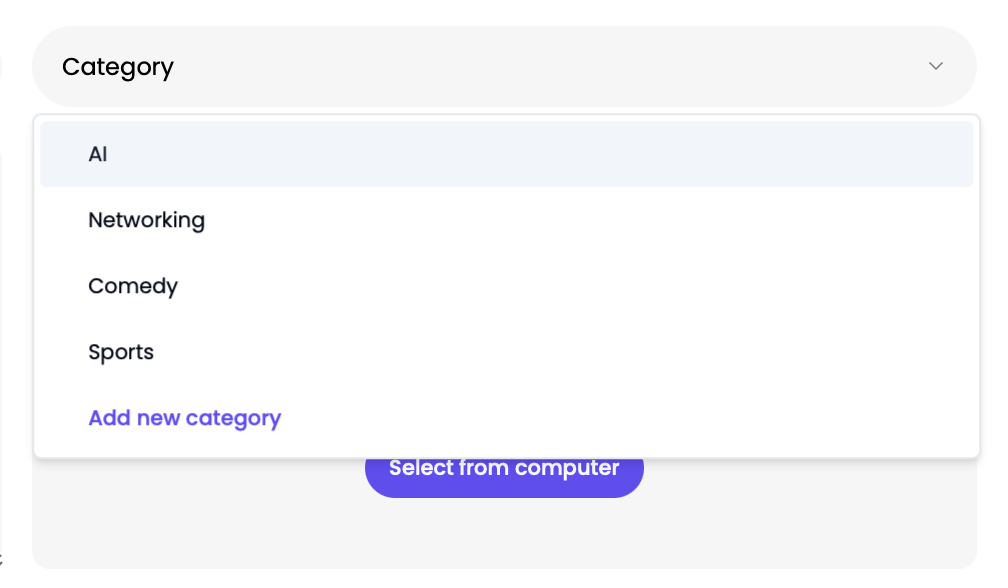
\includegraphics[width=0.6\textwidth,height=200px,frame]{images/createEvent2.png}
	\caption{Create Event - New Category}
        \label{fig:createEvent2}
\end{figure}


The features outlined in this manual are designed to ensure a seamless and intuitive user experience on the platform. By following the instructions in this guide, users can efficiently navigate the website and make the most of its functionalities. Additionally, the detailed sections allow users to troubleshoot and resolve any issues by referring directly to the relevant topics listed in the table of contents.

In the following section, the focus shifts to the \textbf{Developer's Guide}, providing an in-depth explanation of the platform's software implementation. This guide covers both the \textbf{front-end} and \textbf{back-end} systems, offering developers a comprehensive understanding of the platform's architecture, tools, and technologies to assist in further customization and maintenance.




% \begin{table}[H]
% 	\centering
% 	\begin{tabular}{ | m{0.25\textwidth} | m{0.65\textwidth} | }
% 		\hline
% 		\textbf{Phasellus tortor} & \textbf{Aenean consequat} \\
% 		\hline \hline
% 		\emph{Sed malesuada} & Aliquam aliquam velit in convallis ultrices. \\
% 		\hline
% 		\emph{Purus sagittis} &  Quisque lobortis eros vitae urna lacinia euismod. \\
% 		\hline
% 		\emph{Pellentesque} & Curabitur ac lacus pellentesque, eleifend sem ut, placerat enim. Ut auctor tempor odio ut dapibus. \\
% 		\hline
% 	\end{tabular}
% 	\caption{Maecenas tincidunt non justo quis accumsan}
% 	\label{tab:example-1}
% \end{table}

% \subsection{Multi rows and multi columns}

% Mauris a dapibus lectus. Vestibulum commodo nibh ante, ut maximus magna eleifend vel. Integer vehicula elit non lacus lacinia, vitae porttitor dolor ultrices. Vivamus gravida faucibus efficitur. Ut non erat quis arcu vehicula lacinia. Nulla felis mauris, laoreet sed malesuada in, euismod et lacus. Aenean at finibus ipsum. Pellentesque dignissim elit sit amet lacus congue vulputate.

% \begin{table}[htb]
% 	\centering
% 	\begin{tabular}{ | c | r | r | r | r | r | r | }
% 		\hline
% 		\multirow{2}{*}{\textbf{Quisque}} & \multicolumn{2}{ c | }{\textbf{Suspendisse}} & \multicolumn{2}{ c | }{\textbf{Aliquam}} & \multicolumn{2}{ c | }{\textbf{Vivamus}} \\
% 		\cline{2-7}
% 		& Proin & Nunc & Proin & Nunc & Proin & Nunc \\
% 		\hline \hline		
% 		Leo & 2,80 MB & 100\% & 232 KB & 8,09\% & 248 KB & 8,64\% \\
% 		\hline
% 		Vel & 9,60 MB & 100\% & 564 KB & 5,74\% & 292 KB & 2,97\% \\
% 		\hline
% 		Auge & 78,2 MB & 100\% & 52,3 MB & 66,88\% & 3,22 MB & 4,12\% \\
% 		\hline 
% 	\end{tabular}
% 	\caption[Rövid cím a táblázatjegyzékbe]{Vivamus ac arcu fringilla, fermentum neque sed, interdum erat. Mauris bibendum mauris vitae enim mollis, et eleifend turpis aliquet.}
% 	\label{tab:example-2}
% \end{table}

% \subsection{Long tables over multiple pages}

% Nunc porta placerat leo, sit amet porttitor dui porta molestie. Aliquam at fermentum mi. Maecenas vitae lorem at leo tincidunt volutpat at nec tortor. Vivamus semper lacus eu diam laoreet congue. Vivamus in ipsum risus. Nulla ullamcorper finibus mauris non aliquet. Vivamus elementum rhoncus ex ut porttitor.

% \begin{center}
% 	\begin{longtable}{ | p{0.3\textwidth} | p{0.7\textwidth} | }
		
% 		\hline
% 		\multicolumn{2}{|c|}{\textbf{Praesent aliquam mauris enim}}
% 		\\ \hline
		
% 		\emph{Suspendisse potenti} & \emph{Lorem ipsum dolor sit amet}
% 		\\ \hline \hline
% 		\endfirsthead % table header on first page
		
% 		\hline
% 		\emph{Suspendisse potenti} & \emph{Lorem ipsum dolor sit amet}
% 		\\ \hline \hline
% 		\endhead % table header on further pages
		
% 		\hline
% 		\endfoot % table footer on previous pages
		
% 		\endlastfoot % table footer on last page
		
% 		\emph{Praesent}
% 		& Nulla ultrices et libero sit amet fringilla. Nunc scelerisque ante tempus sapien placerat convallis.
% 		\\ \hline
		
% 		\emph{Luctus}
% 		& Integer hendrerit erat massa, non hendrerit risus convallis at. Curabitur ultrices, justo in imperdiet condimentum, neque tortor luctus enim, luctus posuere massa erat vitae nibh.
% 		\\ \hline
		
% 		\emph{Egestas}
% 		& Duis fermentum feugiat augue in blandit. Mauris a tempor felis. Pellentesque ultricies tristique dignissim. Pellentesque aliquam semper tristique. Nam nec egestas dolor. Vestibulum id elit quis enim fringilla tempor eu a mauris. Aliquam vitae lacus tellus. Phasellus mauris lectus, aliquam id leo eget, auctor dapibus magna. Fusce lacinia felis ac elit luctus luctus.
% 		\\ \hline
		
% 		\emph{Dignissim}
% 		& Praesent aliquam mauris enim, vestibulum posuere massa facilisis in. Suspendisse potenti. Nam quam purus, rutrum eu augue ut, varius vehicula tellus. Fusce dui diam, aliquet sit amet eros at, sollicitudin facilisis quam. Phasellus tempor metus vel augue gravida pretium. Proin aliquam aliquam blandit. Nulla id tempus mi. Fusce in aliquam tortor.
% 		\\ \hline
		
% 		\emph{Pellentesque}
% 		& Donec felis nibh, imperdiet a arcu non, vehicula gravida nibh. Quisque interdum sapien eu massa commodo, ac elementum felis faucibus.
% 		\\ \hline
		
% 		\emph{Molestie}
% 		& Cras ullamcorper tellus et auctor ultricies. Maecenas tincidunt euismod lectus nec venenatis. Suspendisse potenti. Pellentesque pretium nunc ut euismod cursus. Nam venenatis condimentum quam. Curabitur suscipit efficitur aliquet. Interdum et malesuada fames ac ante ipsum primis in faucibus.
% 		\\ \hline
		
% 		\emph{Vivamus semper}
% 		& In purus purus, faucibus eu libero vulputate, tristique sodales nunc. Nulla ut gravida dolor. Fusce vel pellentesque mi, vel efficitur eros. Nunc vitae elit tellus. Sed vestibulum auctor consequat. 
% 		\\ \hline
		
% 		\emph{Condimentum}
% 		& Nulla scelerisque, leo et facilisis pretium, risus enim cursus turpis, eu suscipit ipsum ipsum in mauris. Praesent eget pulvinar ipsum, suscipit interdum nunc. Nam varius massa ut justo ullamcorper sollicitudin. Vivamus facilisis suscipit neque, eu fermentum risus. Ut at mi mauris.
% 		\\ \hline
		
% 		\caption{Praesent ullamcorper consequat tellus ut eleifend}
% 		\label{tab:example-3}		
% 	\end{longtable}
% \end{center}
\cleardoublepage




% Define custom colors for code blocks
\definecolor{codegray}{gray}{0.9}
\definecolor{codegreen}{rgb}{0,0.6,0}
\definecolor{codeblue}{rgb}{0,0,0.6}
\definecolor{codepurple}{rgb}{0.58,0,0.82}

% Define custom style for directory listing
\lstdefinelanguage{Tree}{
  moredelim=**[is][\color{blue}]{|}{|}
}

\lstdefinestyle{tree}{
  language=Tree,
  basicstyle=\ttfamily\small,
  showspaces=false,
  showstringspaces=false,
  breaklines=true,
  frame=single,
  backgroundcolor=\color{gray!10},
}


% Define TypeScript as a language
\lstdefinelanguage{typescript}{
  keywords={interface, string, number, boolean, Date, undefined, null, any, void, never, readonly, public, private, protected},
  keywordstyle=\color{codeblue}\bfseries,
  ndkeywords={_id, name, description, location, createdAt, imageUrl, startDateTime, endDateTime, price, isFree, url, category, organizer, stripeId, totalAmount, event, buyer, firstName, lastName, photo, username, clerkId, email},
  ndkeywordstyle=\color{codepurple}\bfseries,
  identifierstyle=\color{black},
  sensitive=true,
  comment=[l]{//},
  morecomment=[s]{/*}{*/},
  commentstyle=\color{codegreen}\ttfamily,
  stringstyle=\color{codepurple}\ttfamily,
  morestring=[b]',
  morestring=[b]"
}

% Set the default style for TypeScript code
\lstdefinestyle{typescript}{
  language=typescript,
  backgroundcolor=\color{codegray},
  basicstyle=\ttfamily\small,
  breaklines=true,
  frame=single,
  numbers=left,
  numberstyle=\tiny\color{gray},
  numbersep=5pt
}
\chapter{Developer documentation}
\label{ch:impl}

This project is designed as a modern \textbf{Next.js full-stack application}, utilizing a monolithic architecture pattern. Instead of separating the front-end and back-end into different repositories, the application consolidates all components into a single repository. 

This architectural choice provides several advantages:

\begin{itemize}
    \item All code resides in a single repository, simplifying development workflows.
    \item Seamless type sharing between client and server components.
    \item Easier deployment and maintenance as a single cohesive unit.
\end{itemize}

\section{Components of design}

\subsection{Use Case Diagram}
The use case diagram represents the interactions between various users of the event management system—\textbf{System Admin}, \textbf{Event Organizer}, and \textbf{Event Attendee}—and the functionalities available to them. Key use cases and relationships include:  

\begin{itemize}
    \item \textbf{Category Management:}  
    The \textbf{System Admin} can manage event categories, such as adding, updating, or removing categories.  

    \item \textbf{Event Management:}  
    \begin{itemize}
        \item The \textbf{Event Organizer} has the ability to create, update, delete, and view events.  
        \item While creating an event, organizers can optionally extend the functionality to include uploading event images or creating new categories.  
        \item Event organizers can also filter and search for events by category.  
    \end{itemize}

    \item \textbf{Order Management:}  
    \begin{itemize}
        \item The \textbf{Event Attendee} can purchase tickets for events and view their orders.  
        \item The purchase ticket flow includes processing payments via an external payment system (e.g., Stripe).  
    \end{itemize}

    \item \textbf{Authentication:}  
    Both \textbf{Event Organizer} and \textbf{Event Attendee} can sign up, sign in, and manage their profiles.  
\end{itemize}

\textbf{Relationships:}  
\begin{itemize}
    \item \textit{Extends:} Optional flows like uploading event images or creating categories are represented as extensions to the main event management flow.  
    \item \textit{Includes:} Common actions like processing payments or uploading files are modularized into reusable flows.  
\end{itemize}

\begin{figure}[H]
	\centering	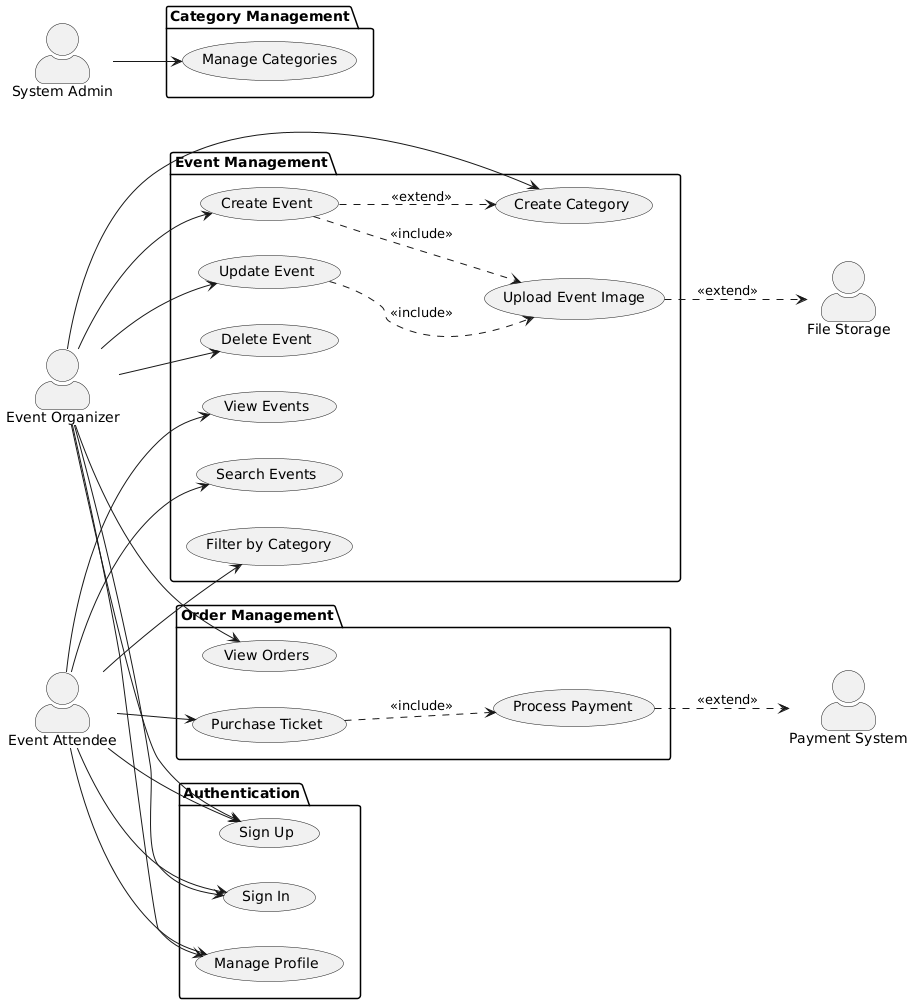
\includegraphics[width=1.0\textwidth,height=500px,frame]{usecase.png}
    \caption{Use Case Diagram}
    \end{figure}


\subsection{UML Class Diagram}  
The UML class diagram provides a clear representation of the core entities in the event management system and their relationships. These entities include \textbf{User}, \textbf{Order}, \textbf{Event}, and \textbf{Category}. The diagram can be summarized as follows:  

\begin{itemize}
    \item \textbf{User:}  
    \begin{itemize}
        \item Fields: \texttt{\_id}, \texttt{clerkId}, \texttt{email}, \texttt{username}, \texttt{firstName}, \texttt{lastName}, \texttt{photo}.  
        \item Represents users in the system and handles authentication and profile management.  
    \end{itemize}
    
    \item \textbf{Order:}  
    \begin{itemize}
        \item Fields: \texttt{\_id}, \texttt{createdAt}, \texttt{stripeId}, \texttt{totalAmount}.  
        \item Represents event bookings and manages payments for tickets.  
    \end{itemize}
    
    \item \textbf{Event:}  
    \begin{itemize}
        \item Fields: \texttt{\_id}, \texttt{title}, \texttt{description}, \texttt{location}, \texttt{createdAt}, \texttt{imageUrl}, \texttt{startDateTime}, \texttt{endDateTime}, \texttt{price}, \texttt{isFree}, \texttt{url}.  
        \item Core entity representing events, including details about location, time, and cost.  
    \end{itemize}
    
    \item \textbf{Category:}  
    \begin{itemize}
        \item Fields: \texttt{\_id}, \texttt{name}.  
        \item Categorizes events into different types (e.g., workshops, concerts).  
    \end{itemize}
\end{itemize}

\textbf{Relationships:}  
\begin{itemize}
    \item \textbf{User-Order:}  
    A user places multiple orders (one-to-many relationship).  
    \item \textbf{User-Event:}  
    A user can organize multiple events (one-to-many relationship).  
    \item \textbf{Event-Category:}  
    Each event belongs to a single category (many-to-one relationship).  
    \item \textbf{Order-Event:}  
    Orders reference specific events (many-to-one relationship).  
\end{itemize}


\begin{figure}[H]
	\centering	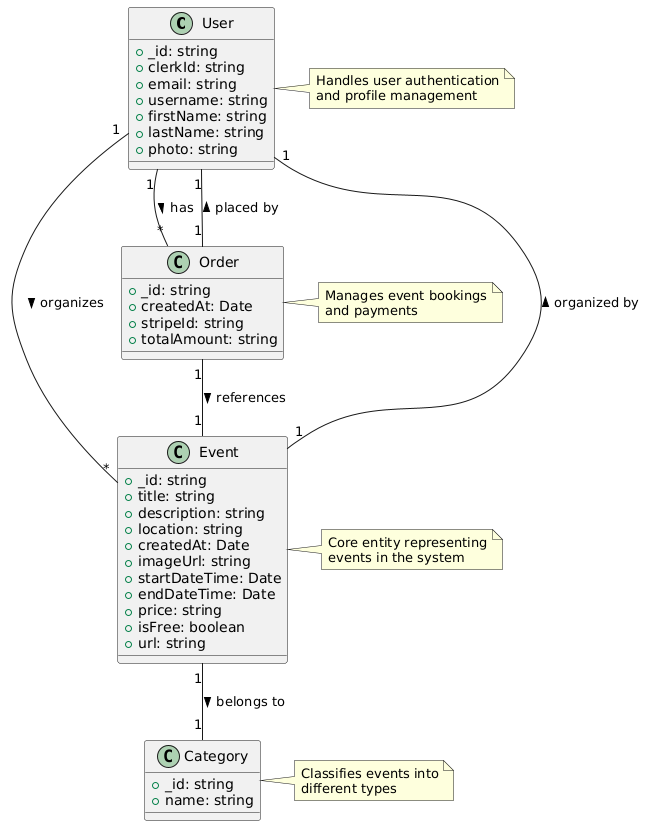
\includegraphics[width=1.0\textwidth,height=500px,frame]{umlclass.png}
    \caption{UML Class Diagram}
    \end{figure}



\subsection{Entity Relationship Diagram (ERD)}

\subsubsection{Overview}
The Event Management Platform's database schema consists of four main entities: \textbf{User}, \textbf{Event}, \textbf{Category}, and \textbf{Order}. The schema is designed to efficiently support event creation, ticket booking, and user management.

\subsubsection{Core Entities}
\paragraph{User}
\begin{itemize}
    \item Stores user profiles and authentication data.
    \item \textbf{Key Fields}: \texttt{id}, \texttt{clerkId}, \texttt{email}, \texttt{username}, \texttt{firstName}, \texttt{lastName}, \texttt{photo}.
    \item Serves as the primary entity for both event organizers and attendees.
\end{itemize}

\paragraph{Event}
\begin{itemize}
    \item Manages event information and scheduling.
    \item \textbf{Key Fields}: \texttt{id}, \texttt{title}, \texttt{description}, \texttt{location}, \texttt{dates}, \texttt{price}, \texttt{imageUrl}.
    \item Links to the event organizer (\texttt{User}) and event category (\texttt{Category}).
\end{itemize}

\paragraph{Category}
\begin{itemize}
    \item Classifies events into various types.
    \item \textbf{Key Fields}: \texttt{id}, \texttt{name}.
    \item Enables event filtering and organization.
\end{itemize}

\paragraph{Order}
\begin{itemize}
    \item Handles ticket purchases and payment processing.
    \item \textbf{Key Fields}: \texttt{id}, \texttt{stripeId}, \texttt{totalAmount}, \texttt{createdAt}.
    \item Links the buyer (\texttt{User}) with the purchased \texttt{Event}.
\end{itemize}

\subsubsection{Key Relationships}
\begin{itemize}
    \item \textbf{User $\rightarrow$ Event (1:N)}: A user can organize multiple events.
    \item \textbf{User $\rightarrow$ Order (1:N)}: A user can make multiple ticket purchases (orders).
    \item \textbf{Event $\rightarrow$ Category (N:1)}: Each event belongs to one category.
    \item \textbf{Event $\rightarrow$ Order (1:N)}: An event can have multiple ticket orders.
\end{itemize}

\subsubsection{Implementation}
\begin{itemize}
    \item The database is built using \textbf{MongoDB} with \textbf{Mongoose ODM}.
    \item Referential integrity is implemented through \texttt{ObjectId} references.
    \item Designed to support efficient querying and data retrieval.
    \item Validation rules and required field constraints are included to ensure data consistency.
\end{itemize}

\begin{figure}[H]
	\centering	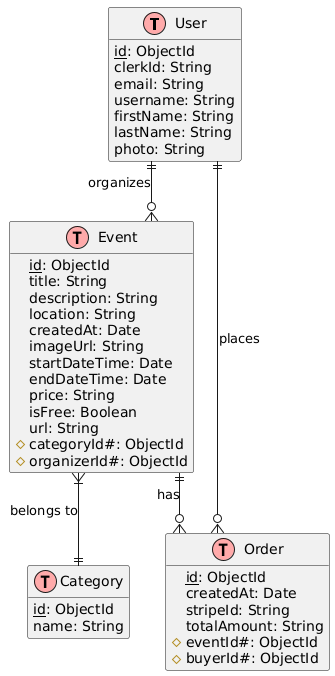
\includegraphics[width=0.6\textwidth,height=450px,frame]{erd.png}
    \caption{Entity Relationship Diagram}
    \end{figure}





\subsection{User Sequence Diagram}

The sequence diagram illustrates the interaction flow between the system components and the user, highlighting key processes such as authentication, event creation, booking, and management. Below is an explanation of each sequence:

\begin{itemize}
    \item \textbf{User Authentication:}
    \begin{itemize}
        \item The user initiates the process by accessing the platform.
        \item The frontend (Next.js) sends a request for authentication to the authentication service (Clerk Auth).
        \item The authentication service returns the session details. For new users, the process involves creating a user record in the database via a webhook triggered by \texttt{user.created}, confirming creation, and updating the user metadata.
    \end{itemize}

    \item \textbf{Event Creation:}
    \begin{itemize}
        \item The user begins the process of creating a new event via the frontend.
        \item An image for the event is uploaded to a file storage service (UploadThing), which returns the image URL.
        \item Event details are then submitted to the backend, where they are stored in the database (MongoDB), and the system confirms the successful storage of data.
        \item The user is shown a success confirmation on the frontend.
    \end{itemize}

    \item \textbf{Event Booking:}
    \begin{itemize}
        \item The user clicks on "Book Event," initiating a checkout session via the backend.
        \item The backend communicates with Stripe to create a session and returns the session URL to the frontend, redirecting the user to the Stripe payment page.
        \item Two possible scenarios:
        \begin{itemize}
            \item \textit{Successful Payment:} Stripe triggers a webhook for payment success. The backend creates an order record in the database, confirms the order and the user is shown a success page.
            \item \textit{Payment Failed:} The user is shown an error message in case of failure.
        \end{itemize}
    \end{itemize}

    \item \textbf{Event Management:}
    \begin{itemize}
        \item The user accesses their dashboard to manage events.
        \item The frontend requests the user's events from the backend.
        \item The backend queries the database for the events and returns the data.
        \item The user is presented with a list of their events.
    \end{itemize}
\end{itemize}


\begin{figure}[H]
	\centering	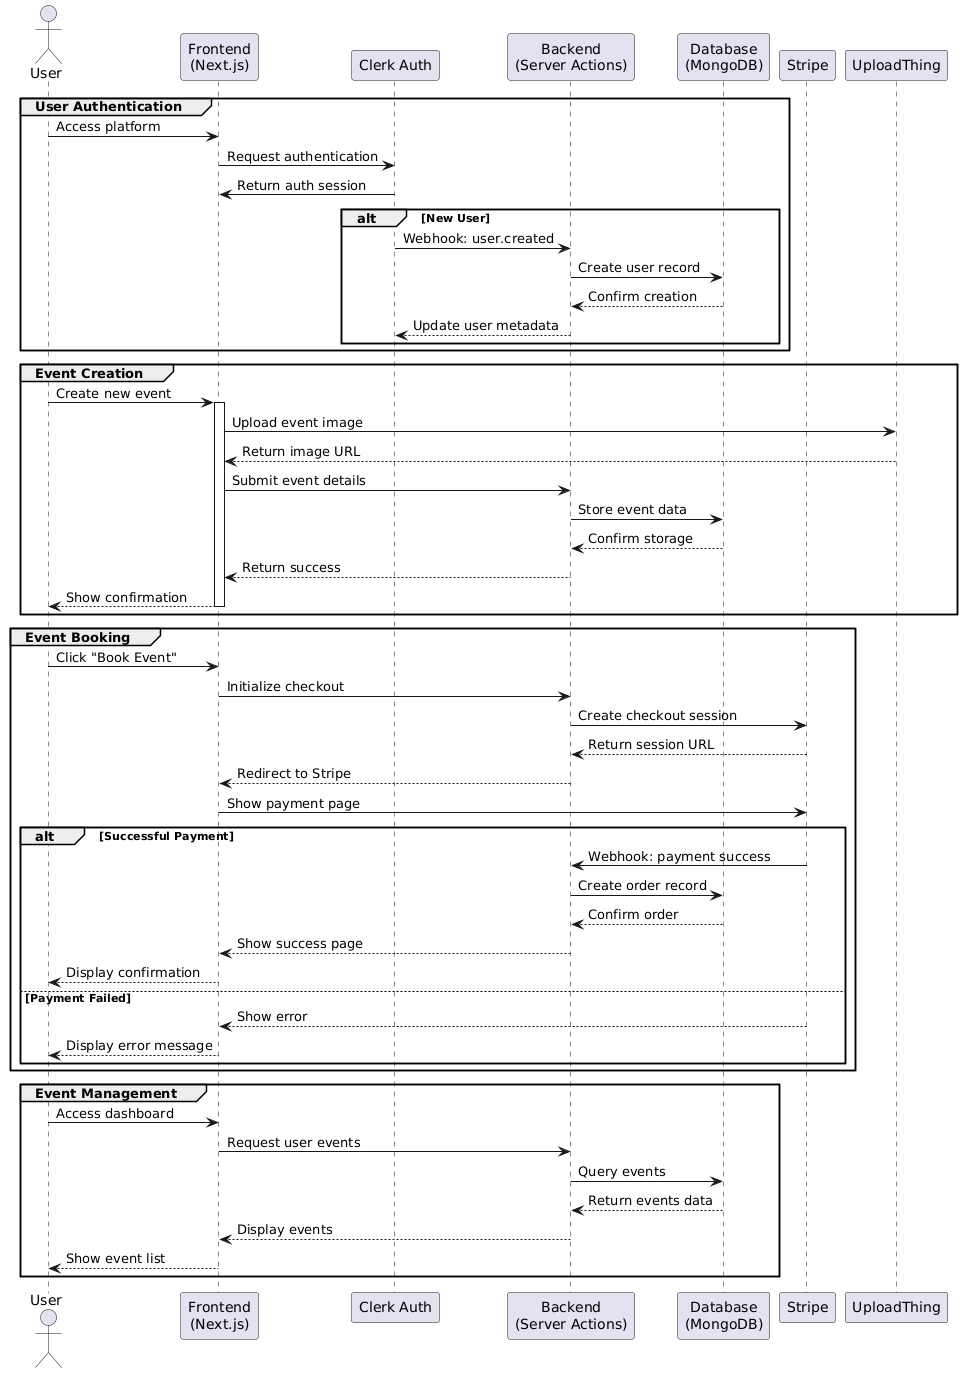
\includegraphics[width=1.0\textwidth,height=700px,frame]{userseq.png}
    \caption{User Sequence Diagram}
    \end{figure}




\section{Implementation}

The technology stack for this project is composed of:

\paragraph{Frontend Technologies}
\begin{itemize}
    \item \textbf{Next.js 14}: Core framework providing both client and server capabilities.
    \item \textbf{TypeScript}: For type-safe code development.
    \item \textbf{Tailwind CSS}: For responsive and utility-first styling.
    \item \textbf{React Hook Form}\cite{reacthookform}: Form management and validation.
    \item \textbf{Zod}\cite{zod}: Schema validation library.
    \item \textbf{RadixUI}\cite{radixui}: Accessible component primitives.
    \item \textbf{React DatePicker}\cite{reactdatepicker}: Date and time selection component.
\end{itemize}

\paragraph{Backend Technologies}
\begin{itemize}
    \item \textbf{MongoDB}: NoSQL database for flexible data storage.
    \item \textbf{Mongoose}: ODM (Object Data Modeling) for MongoDB interaction.
    \item \textbf{Clerk}: Authentication and user management.
    \item \textbf{Stripe}: Payment processing integration.
    \item \textbf{Uploadthing}: File upload and storage solution.
\end{itemize}


\subsection{Hardware Requirements}
Hardware requirements are highly subjective. Most modern computers can handle a medium-sized web project. However, the following specifications are recommended for optimal performance:

\begin{itemize}
    \item \textbf{Processor:} Multi-core CPU
    \item \textbf{RAM:} At least 8 GB
    \item \textbf{Storage:} SSD with at least 256 GB of free space
    \item \textbf{Operating System:} Modern 64-bit OS
\end{itemize}


\subsection{Software Requirements}

The following is the list of software tools used in the development process. After the list, the setup and usage for each of them will be explained.

\begin{itemize}
    \item \textbf{Node.js (v20.12.2):} Used for running the Next.js application.
    \item \textbf{MongoDB:} NoSQL database for flexible and efficient data storage.
    \item \textbf{Stripe:} Payment processing for ticket purchases.
    \item \textbf{Uploadthing:} File upload and storage solution for event images.
    \item \textbf{Clerk:} Authentication and user management.
    \item \textbf{Git:}\cite{git} Version control system for tracking code changes.
\end{itemize}



\subsection{Software Environment Set up}
This section provides detailed instructions on how to install and set up the required software step by step. Please follow these instructions carefully. Once these steps are completed successfully, the development environment will be ready to use.

\begin{enumerate}
    \item \textbf{Node.js Setup:}
    \begin{itemize}
        \item Download the latest stable version of Node.js from \texttt{https://nodejs.org}.
        \item Install it following the on-screen instructions.
        \item Verify installation by running \texttt{node -v} and \texttt{npm -v} in your terminal.
    \end{itemize}
    
    \item \textbf{MongoDB:}
    \newline
    To store data for the application, it is essential to have a MongoDB account and configure the connection URL provided by MongoDB. Follow the steps below to set up MongoDB for your project:
    \begin{enumerate}
    \item \textbf{Create a MongoDB Account:}
    \begin{itemize}
        \item Register an account at \url{https://mongodb.com}.
        \item After logging in, you will be redirected to \url{https://cloud.mongodb.com}.
    \end{itemize}
    
    \item \textbf{Create a Database:}
    \begin{itemize}
        \item Navigate to the \textit{Database} tab.
        \item Click on \textit{Create Database} and follow the prompts as shown in Figure~\ref{fig:create_database}.
    \end{itemize}

    \begin{figure}[H]
	\centering	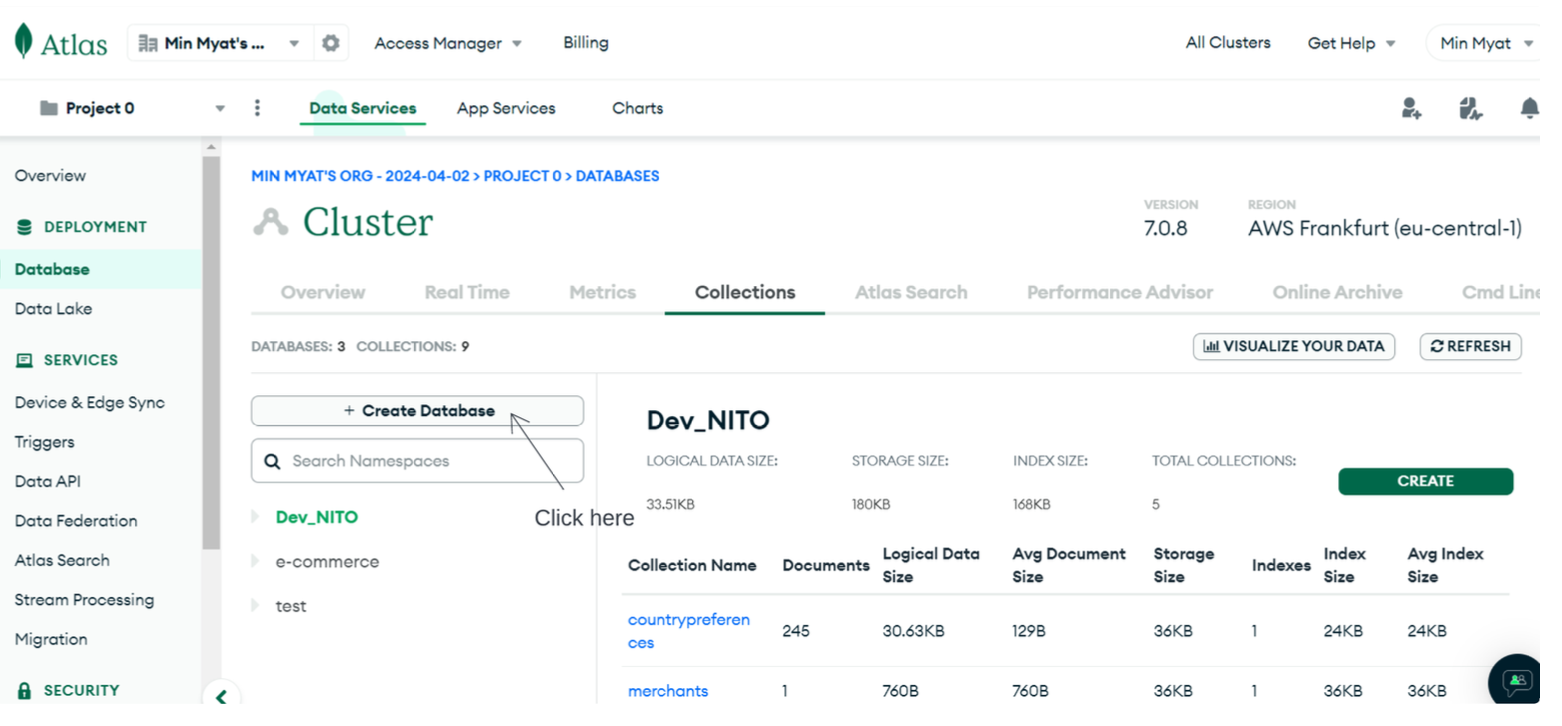
\includegraphics[width=1.0\textwidth,height=300px,frame]{create_database_example.png}
    \caption{How to Create a Database}
    \label{fig:create_database}
    \end{figure}

    \item \textbf{Connect to the Database:}
    \begin{itemize}
        \item Navigate to the \textit{Overview} tab on the left side.
        \item Click on the \textit{Connect} button (see Figure~\ref{fig:connect_database}).
        \item A modal with connection instructions will appear.
    \end{itemize}

    \begin{figure}[H]
	\centering	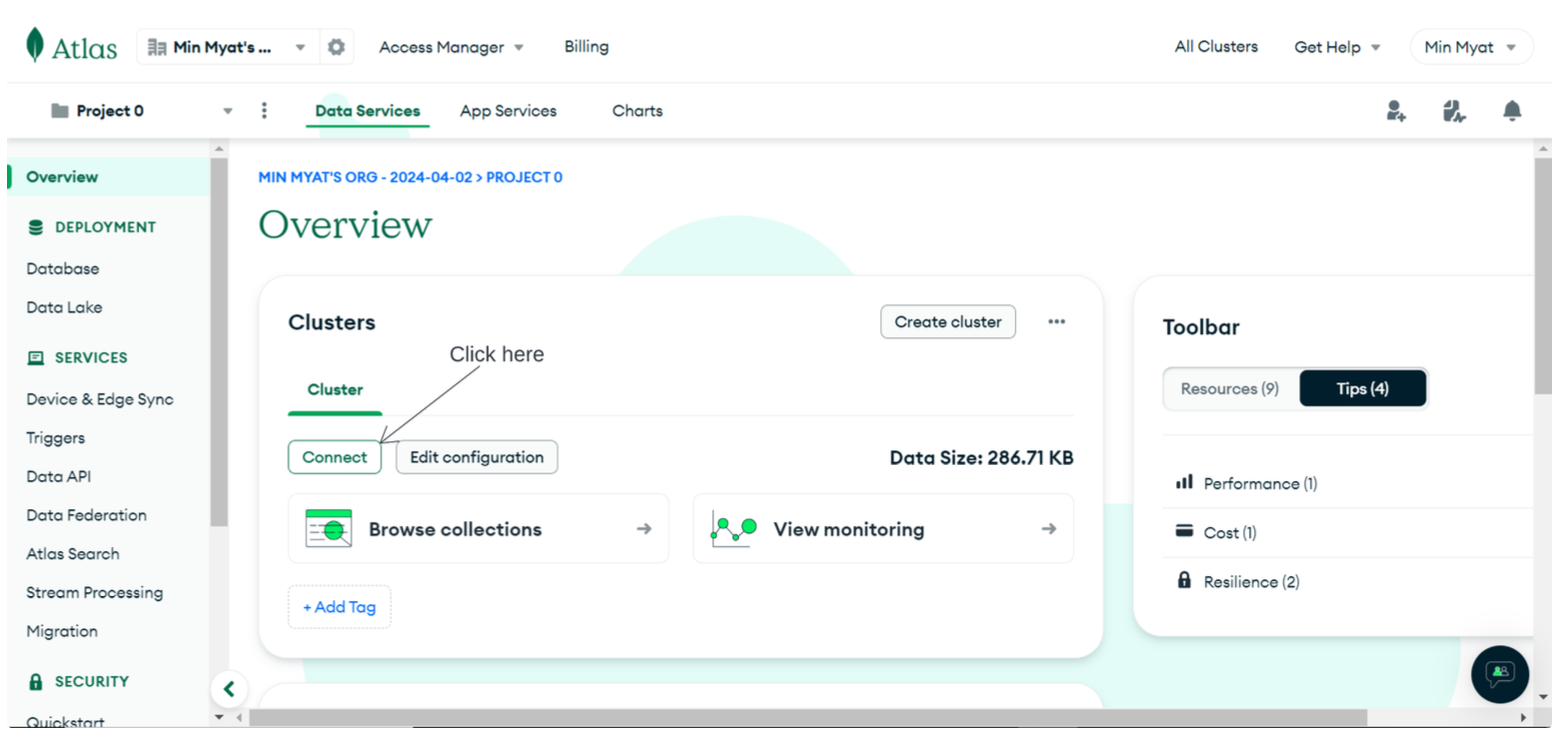
\includegraphics[width=1.0\textwidth,height=300px,frame]
    {connect_database_example.png}
    \caption{How to Connect to the Database}
    \label{fig:connect_database}
    \end{figure}
    
    
    \item \textbf{Modify the Connection String:}
    \begin{itemize}
        \item Copy the connection string provided by MongoDB.
        \item Replace the placeholders in the connection string with your username, password, and database name. Below is an example:
        \lstset{caption={MONGODB connection string}}
\begin{lstlisting}
const url = "mongodb+srv://<username>:<password>
        @cluster0.2cqmiec.mongodb.net/<database-name>?
        retryWrites=true&w=majority&appName=<cluster-name>"
\end{lstlisting}
        \item If the cluster name was customized, it can be found in the \textit{Cluster Name} section (see Figure~\ref{fig:cluster_name}).
    \end{itemize}

    \begin{figure}[H]
	\centering	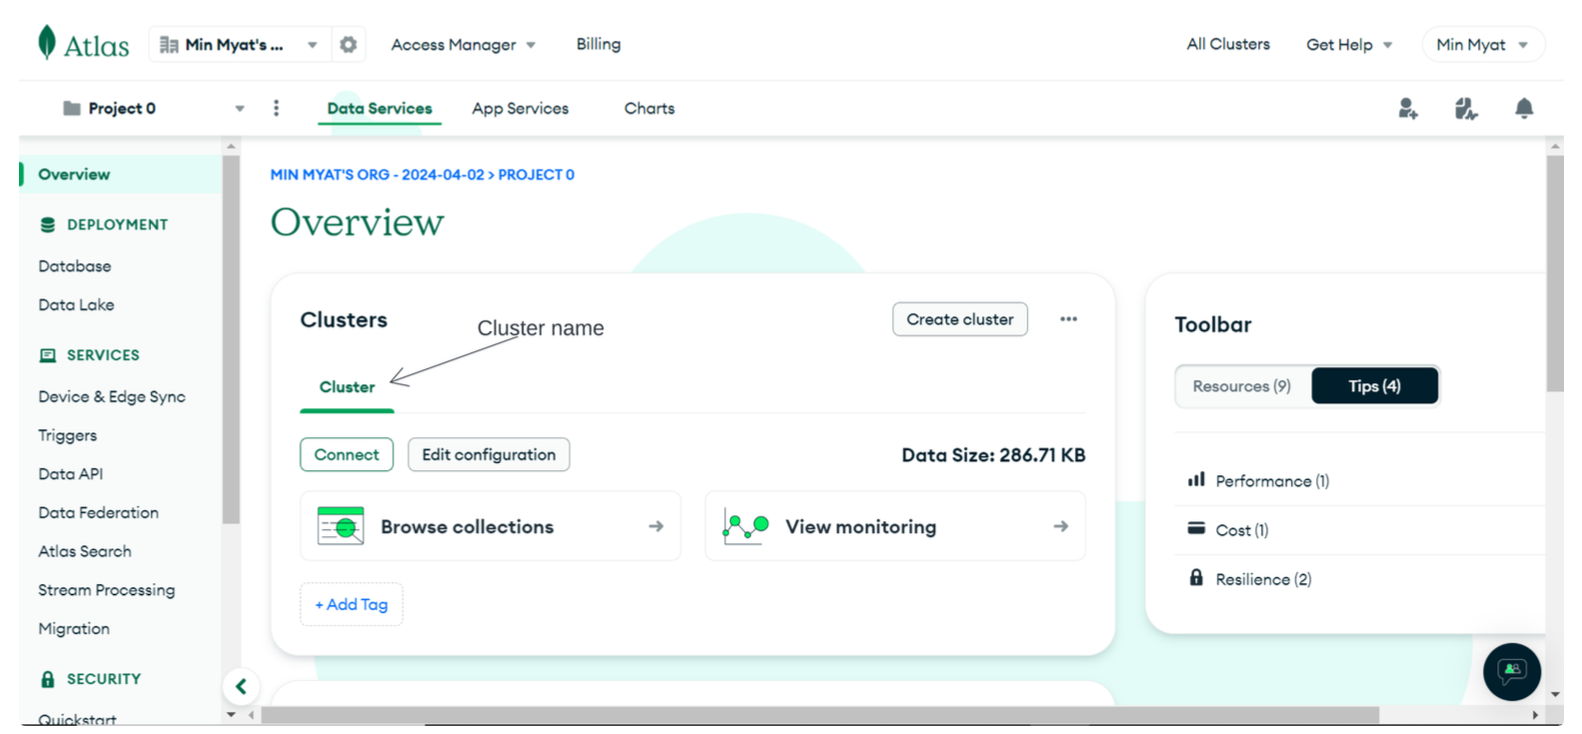
\includegraphics[width=1.0\textwidth,height=300px,frame]{cluster_name_example.png}
    \caption{How to Find Cluster Name}
    \label{fig:cluster_name}
    \end{figure}

    
    \item \textbf{Save the Connection String:}
    \begin{itemize}
        \item Store the modified connection string in the \texttt{.env} file as follows:
        
        \begin{verbatim}
        MONGO_DB_URL="your_connection_string_here"
        \end{verbatim}
    \end{itemize}
\end{enumerate}

Once these steps are completed, your database is ready for data input and output.






    \item \textbf{Stripe Integration:}
    \begin{itemize}
        \item Create an account at \texttt{https://stripe.com}.
        \item Obtain your API keys from the dashboard (see Figure~\ref{fig:stripe_api}).
        \item Configure the keys in your environment variables.
    \end{itemize}
    \begin{figure}[H]
	\centering	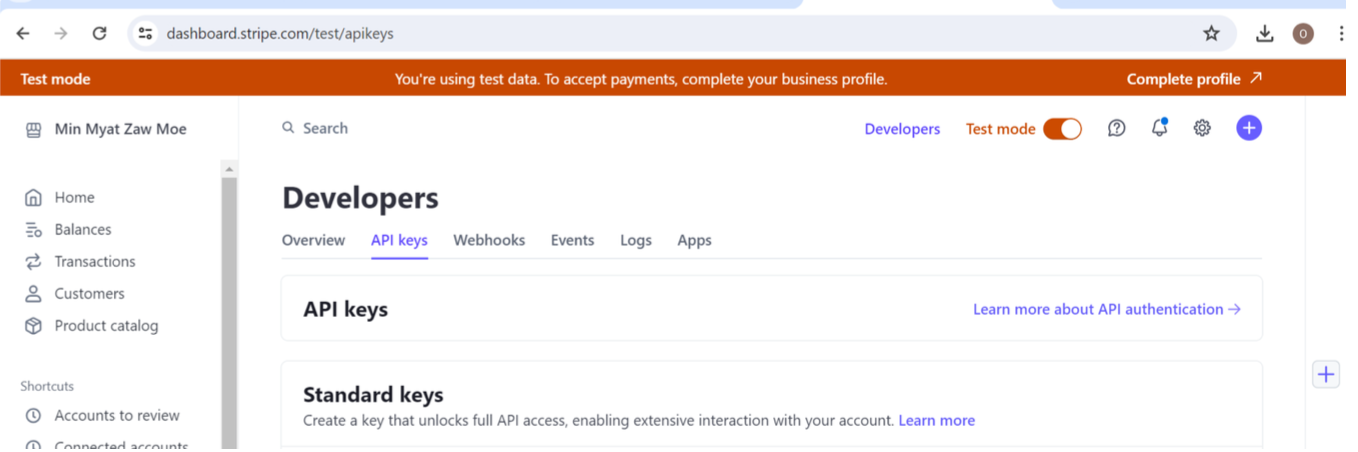
\includegraphics[width=1.0\textwidth,height=200px,frame]
    {stripeAPI.png}
    \caption{Stripe API Key}
    \label{fig:stripe_api}
    \end{figure}

    \item \textbf{Uploadthing Setup:}
    \begin{itemize}
        \item Sign up and create an account at \texttt{https://uploadthing.com}.
        \item Obtain your API key and configure it in the environment variables (see Figure~\ref{fig:ut_api}).
    \end{itemize}
    \begin{figure}[H]
	\centering	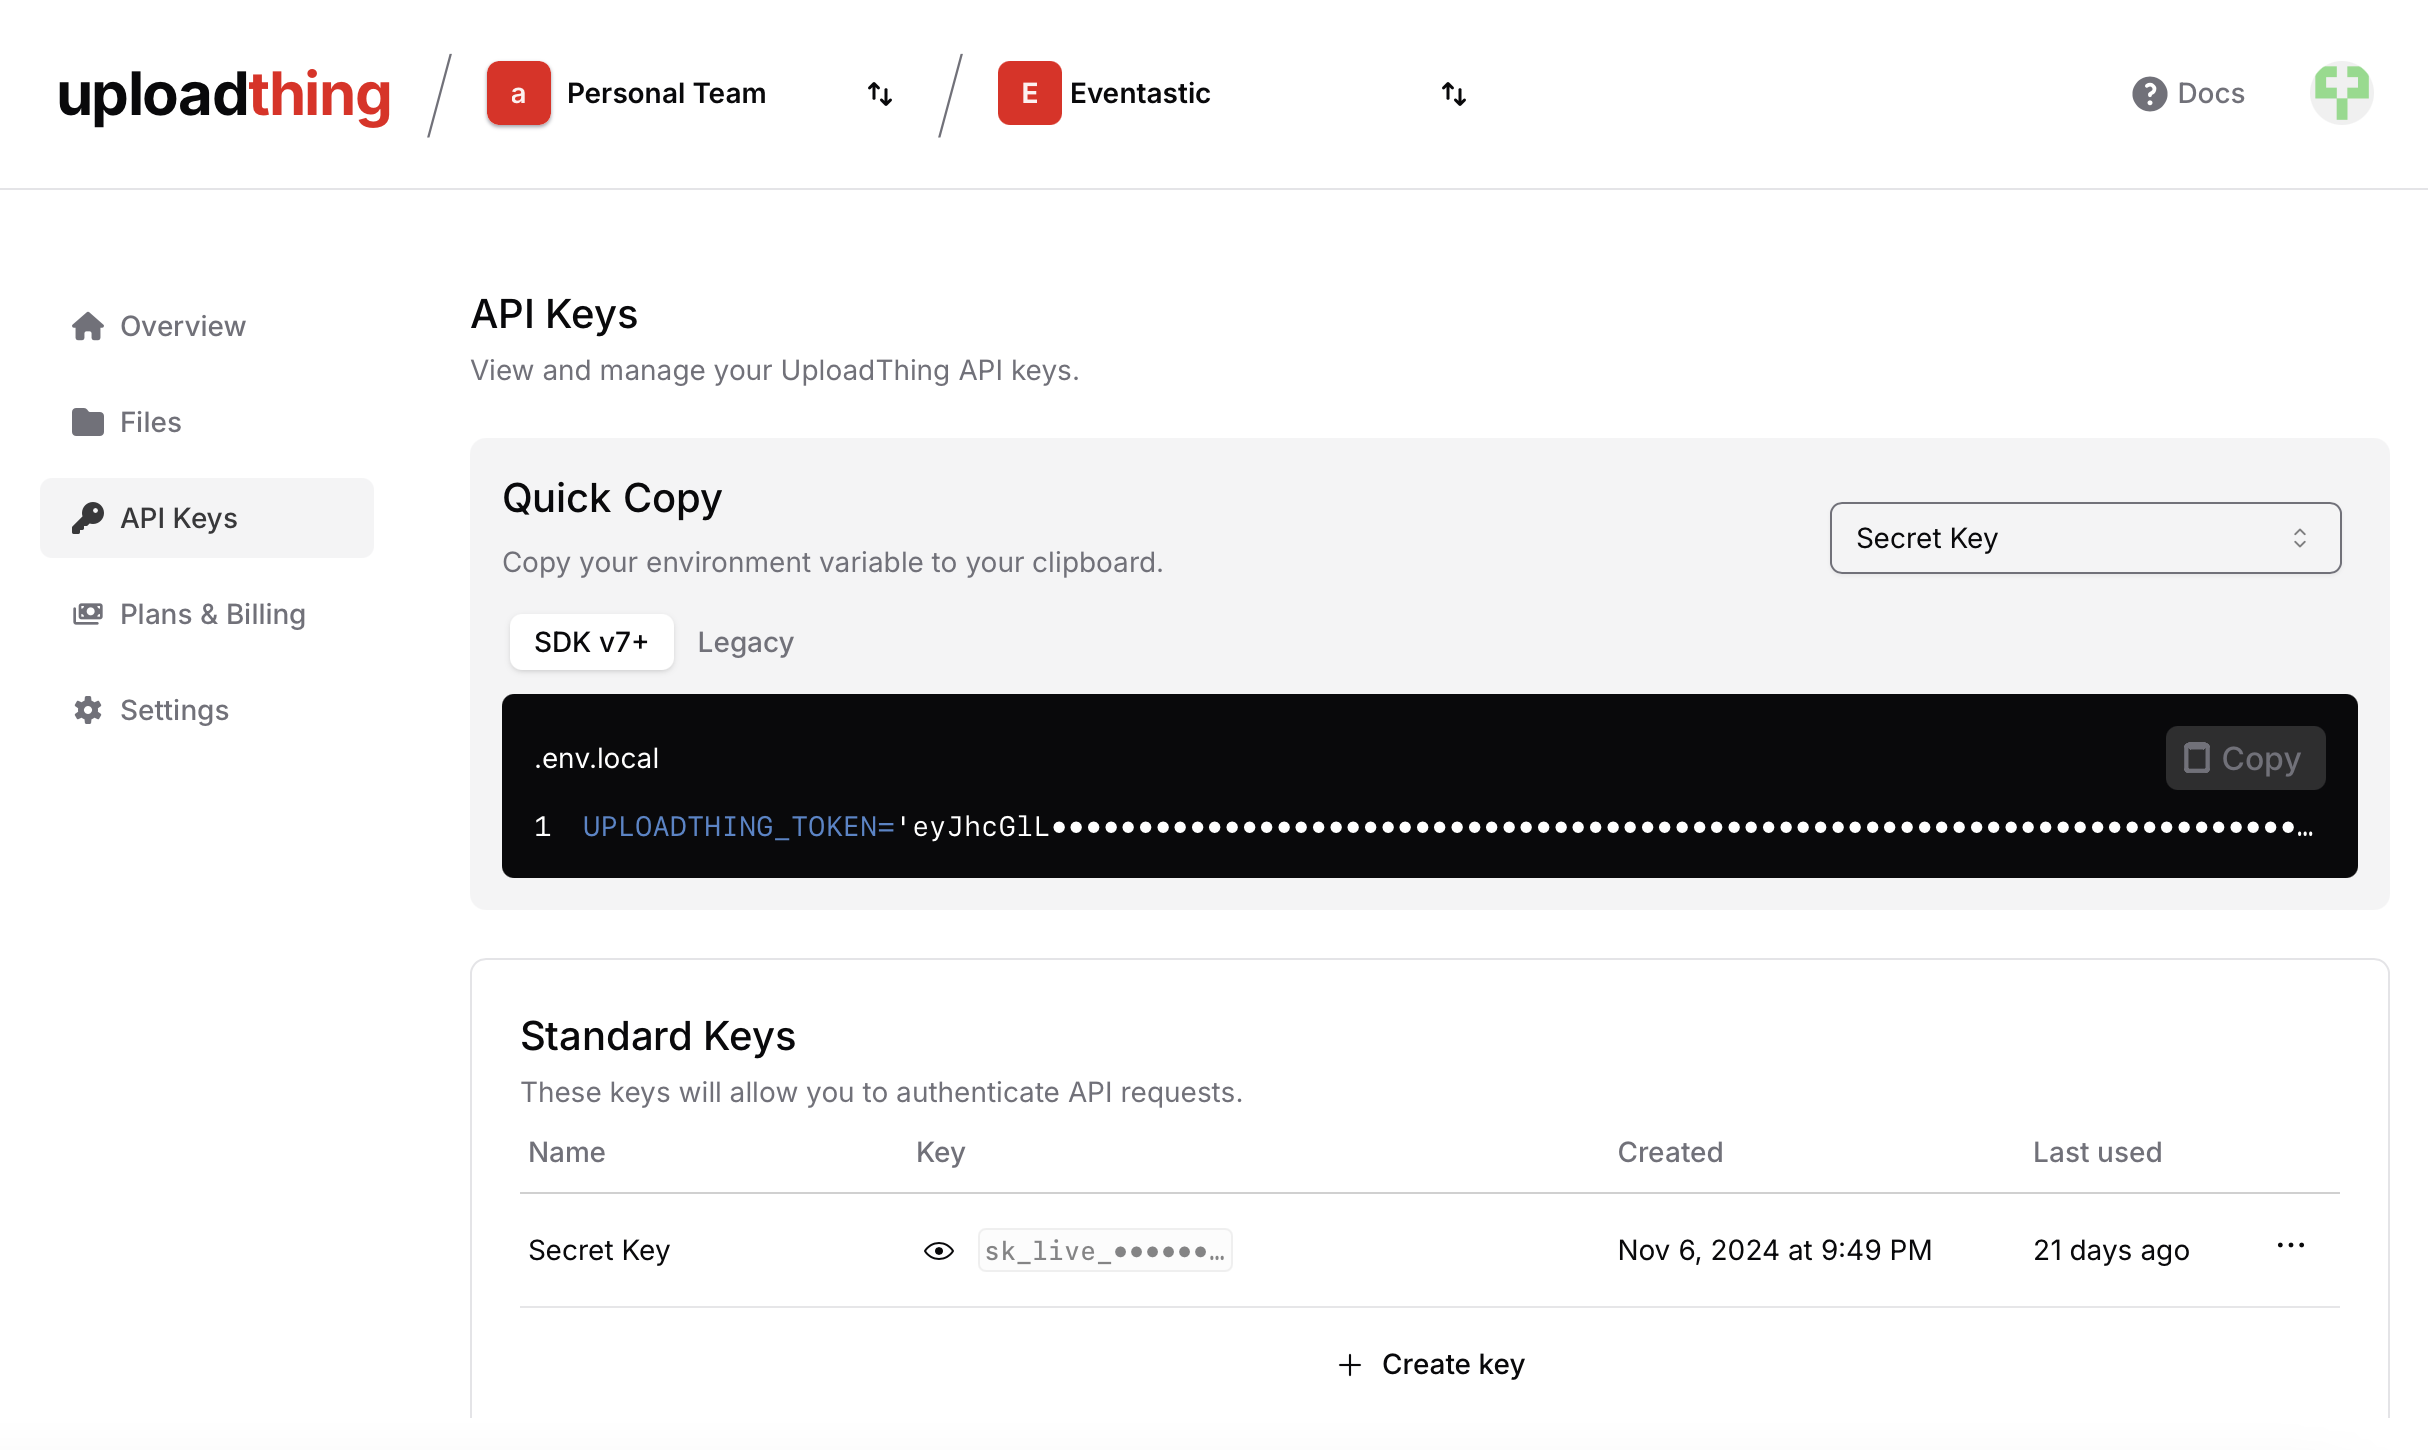
\includegraphics[width=1.0\textwidth,height=300px,frame]
    {utAPI.png}
    \caption{UploadThing API Key}
    \label{fig:ut_api}
    \end{figure}
    

    \item \textbf{Clerk Authentication:}
    \begin{itemize}
        \item Create an account at \texttt{https://clerk.dev}.
        \item Set up your application in the Clerk dashboard.
        \item Configure the required API keys in the environment file (see Figure~\ref{fig:clerk_api})).
    \end{itemize}
    \begin{figure}[H]
	\centering	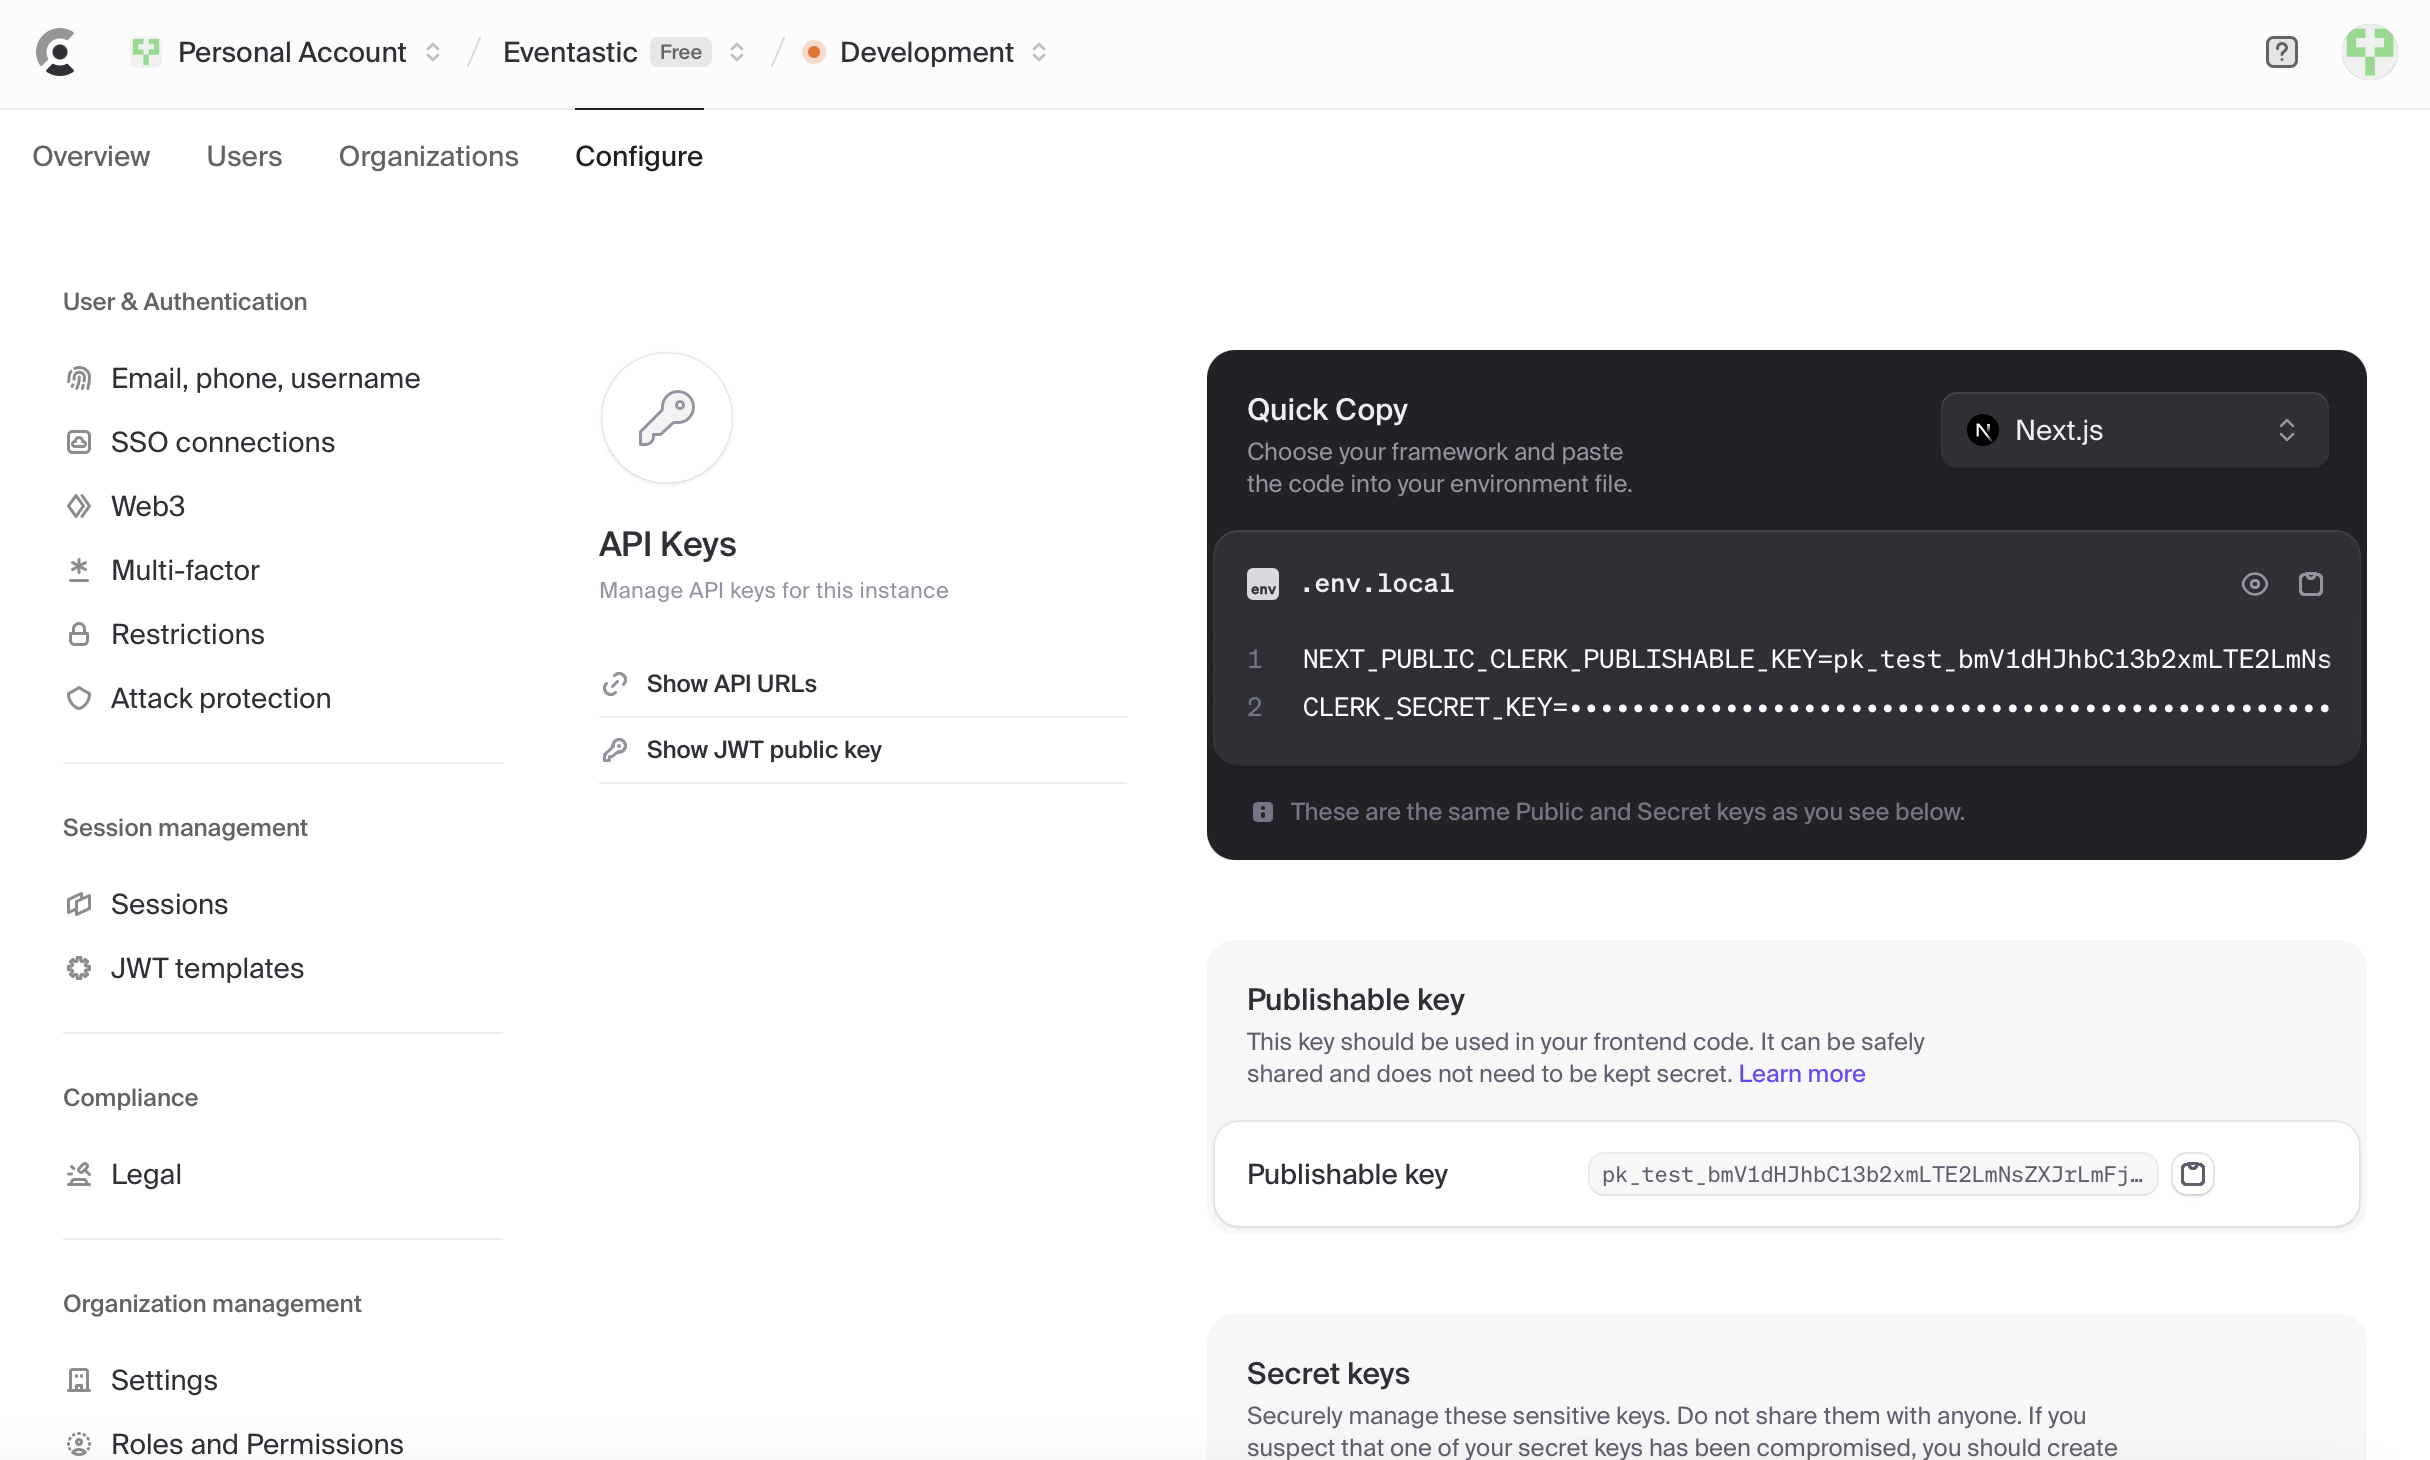
\includegraphics[width=1.0\textwidth,height=300px,frame]
    {clerkAPI.png}
    \caption{Clerk API Key}
    \label{fig:clerk_api}
    \end{figure}

    \item \textbf{Postman:}\cite{postman}
    \begin{itemize}
        \item Download Postman from \texttt{https://www.postman.com/downloads/}.
        \item Install and log in to start testing APIs.
    \end{itemize}

    \item \textbf{Git Setup:}
    \begin{itemize}
        \item Install Git from \texttt{https://git-scm.com/downloads}.
        \item Configure your username and email with the following commands:
        \begin{verbatim}
        git config --global user.name "Your Name"
        git config --global user.email "your.email@example.com"
        \end{verbatim}
    \end{itemize}
\end{enumerate}



If the reader has followed the steps outlined above, the development process can now begin. However, before diving into development, it is crucial to first understand the data models used in the application.

By familiarizing yourself with the data schema, you will gain a deeper insight into the workings of the API and the data presentation layers. This understanding will help clarify:
\begin{itemize}
    \item The structure and types of data being sent in API requests.
    \item The expected format and content of API responses.
\end{itemize}

This foundational knowledge will streamline your development efforts and ensure a more efficient interaction with the application’s backend services.






\section{Data Models}

This section provides a detailed overview of the data models used in the application.

\subsection{Category Model}

The \textbf{Category} model represents categories for events.

\begin{lstlisting}[style=typescript, caption={Category Model Interface}]
interface ICategory {
  _id: string;
  name: string;
}

Schema:
- _id: MongoDB ObjectId
- name: String (required)
\end{lstlisting}


\subsection{Event Model}

The \textbf{Event} model represents events in the system.

\begin{lstlisting}[style=typescript, caption={Event Model Interface}]
interface IEvent {
  _id: string;
  title: string;
  description?: string;
  location?: string;
  createdAt: Date;
  imageUrl: string;
  startDateTime: Date;
  endDateTime: Date;
  price: string;
  isFree: boolean;
  url?: string;
  category: { _id: string; name: string };
  organizer: { _id: string; firstName: string; lastName: string };
}

Schema:
- _id: MongoDB ObjectId
- title: String (required)
- description: String
- location: String
- createdAt: Date (default: Date.now)
- imageUrl: String (required)
- startDateTime: Date (required)
- endDateTime: Date (required)
- price: String (required)
- isFree: Boolean (required)
- url: String
- category: Reference to Category model
- organizer: Reference to User model
\end{lstlisting}


\subsection{Order Model}

The \textbf{Order} model represents event orders/tickets.

\begin{lstlisting}[style=typescript, caption={Order Model Interface}]
interface IOrder {
  _id: string;
  createdAt: Date;
  stripeId: string;
  totalAmount: string;
  event: { _id: string; title: string };
  buyer: { _id: string; firstName: string; lastName: string };
}

interface IOrderItem {
  _id: string;
  eventId: string;
  buyerId: string;
  totalAmount: string;
  createdAt: Date;
  stripeId: string;
}

Schema:
- _id: MongoDB ObjectId
- createdAt: Date (default: Date.now)
- stripeId: String (required)
- totalAmount: String (required)
- event: Reference to Event model
- buyer: Reference to User model
\end{lstlisting}

\subsection{User Model}

The \textbf{User} model represents user accounts in the system.

\begin{lstlisting}[style=typescript, caption={User Model Interface}]
interface IUser {
  _id: string;
  clerkId: string;
  email: string;
  username: string;
  firstName: string;
  lastName: string;
  photo: string;
}

Schema:
- _id: MongoDB ObjectId
- clerkId: String (unique, required)
- email: String (unique, required)
- username: String (unique, required)
- firstName: String (required)
- lastName: String (required)
- photo: String (required)
\end{lstlisting}

\subsection{Database Information}

The application uses \textbf{MongoDB} as its database, utilizing \textbf{Mongoose} as the ODM (Object Document Mapper). Each model is defined with TypeScript interfaces for type safety and Mongoose schemas for database structure. The models are interconnected through references, creating a relational structure within the MongoDB document database.


\section{Program}

The project leverages the \textbf{Next.js App Router} to maintain a clear structure and separation of concerns:
\begin{itemize}
    \item \texttt{app/}: Contains all page components and routing logic.
    \item \texttt{components/}: Houses reusable UI components.
    \item \texttt{lib/}: Includes server-side business logic and database interactions.
    \item \texttt{api/}: Defines API routes for external integrations.
\end{itemize}


While the codebase is not physically divided into separate repositories, it adheres to clear boundaries for maintainability:
\begin{itemize}
    \item \textbf{Front-end concerns}: Managed within the \texttt{app/} and \texttt{components/} directories.
    \item \textbf{Back-end logic}: Encapsulated within \texttt{lib/} and \texttt{api/}.
    \item \textbf{Database models}: Isolated in \texttt{lib/database/models/}.
    \item \textbf{Business logic actions}: Grouped within \texttt{lib/actions/}.
\end{itemize}



\subsection{Folder Structure}
The project follows a modern Next.js 14 application structure\cite{nextjs_project_structure} with a clear separation of concerns. Here's a detailed breakdown of the project organization:

\subsubsection{Root Directory Structure}

\begin{figure}[H]
	\centering	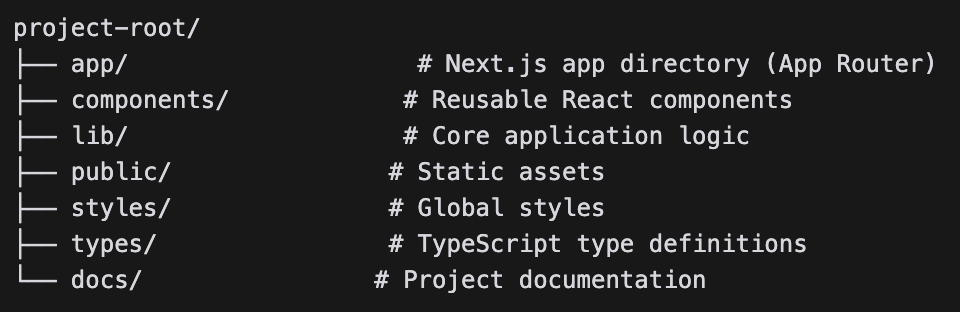
\includegraphics[width=1.0\textwidth,height=140px,frame]{rootdir.png}
    \caption{Root Directory Structure}
    \end{figure}


\subsubsection{Detailed Structure}

\begin{itemize}
    \item \textbf{App Directory (\texttt{/app})} \\
    The app directory utilizes Next.js 14 App Router architecture with the following structure: 
    \begin{figure}[H]
        \centering
        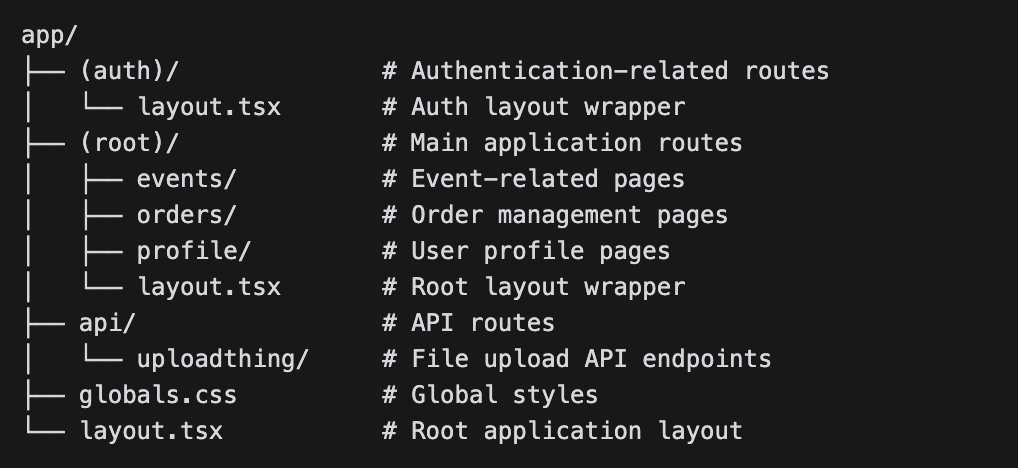
\includegraphics[width=1.0\textwidth,height=200px,frame]{appdir.png}
        \caption{App Directory Structure}
    \end{figure}

    \item \textbf{Components Directory (\texttt{/components})} \\
    The components directory contains reusable UI components:
    \begin{figure}[H]
        \centering
        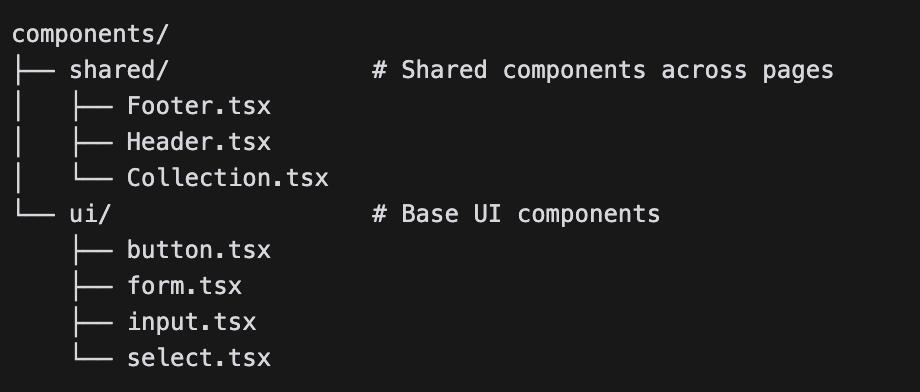
\includegraphics[width=1.0\textwidth,height=190px,frame]{componentsdir.png}
        \caption{Components Directory Structure}
    \end{figure}

    \item \textbf{Library Directory (\texttt{/lib})} \\
    The library directory includes utility functions and libraries:
    \begin{figure}[H]
        \centering
        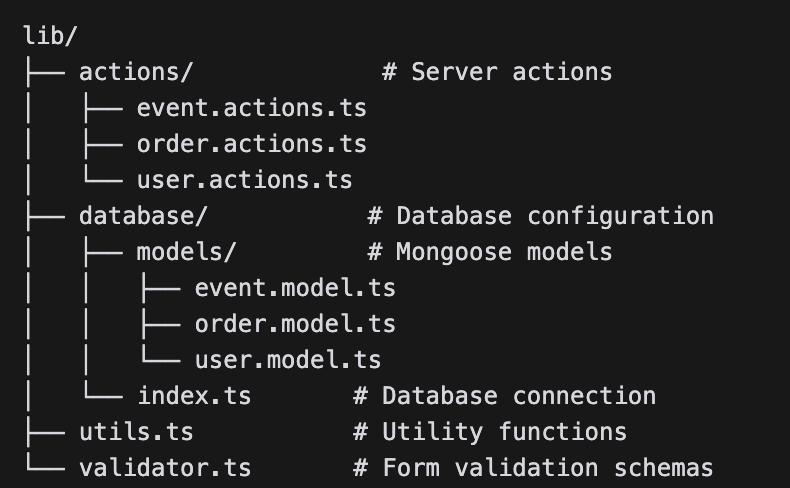
\includegraphics[width=1.0\textwidth,height=190px,frame]{libdir.png}
        \caption{Library Directory Structure}
    \end{figure}

    \item \textbf{Configuration Files} \\
    Key configuration files are located in the root directory:
    \begin{figure}[H]
        \centering
        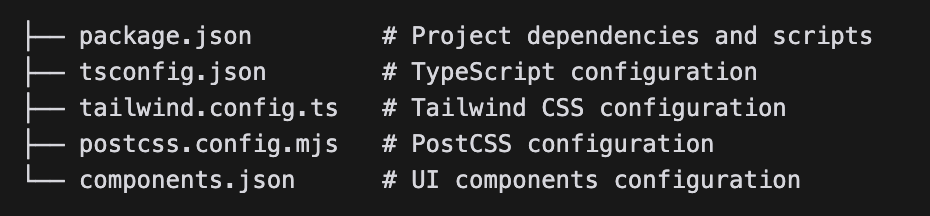
\includegraphics[width=1.0\textwidth,height=100px,frame]{configdir.png}
        \caption{Configuration Files}
    \end{figure}
\end{itemize}


\subsection{User Authentication System}
The application uses Clerk as its authentication provider, offering a robust and secure user management system. This integration provides a seamless authentication experience with features like email verification, social logins, and secure session management.

\subsubsection{Authentication Setup}
The project implements authentication using the following key components:
\begin{itemize}
    \item \textbf{Clerk Provider Configuration} 
\begin{lstlisting}[style=typescript, caption={Clerk Provider Configuration}]
    <ClerkProvider>
      <html lang="en">
        <body className={poppins.variable}>{children}</body>
      </html>
    </ClerkProvider>
  )
\end{lstlisting}

    \item \textbf{Protected Routes}  
    The middleware configuration controls access to different parts of the application:
\begin{lstlisting}[style=typescript, caption={middleware configuration routes}]
import { authMiddleware } from "@clerk/nextjs";
 
export default authMiddleware({
  publicRoutes: [
    '/',
    '/events/:id',
    '/api/webhook/clerk',
    '/api/webhook/stripe',
    '/api/uploadthing'
  ],
  ignoredRoutes: [
    '/api/webhook/clerk',
    '/api/webhook/stripe',
    '/api/uploadthing'
  ]
});
\end{lstlisting}


    
\end{itemize}


\subsubsection{User Registration Flow}
\begin{itemize}
    \item \textbf{Sign-Up Process}
    \begin{itemize}
    \item \textbf{Implemented through Clerk's built-in UI components:} Provides a pre-designed and customizable user interface for handling authentication workflows.
    \item \textbf{Automatic Email Verification:} Clerk handles email verification seamlessly without additional backend logic.
    \item \textbf{User Record Creation:} Upon successful registration, a webhook triggers the creation of a new user record in MongoDB.
    \item \textbf{Integration with Clerk:} Links the Clerk ID to the internal user database for consistent authentication and user profile management.
\end{itemize}

    \item \textbf{User Data Management}  
    When a new user registers, the system creates a user record in MongoDB with the following structure:
\begin{lstlisting}[style=typescript, caption={User Data Management}]
const UserSchema = new Schema({
  clerkId: { type: String, required: true, unique: true },
  email: { type: String, required: true, unique: true },
  username: { type: String, required: true, unique: true },
  firstName: { type: String, required: true },
  lastName: {type: String, required: true },
  photo: { type: String, required: true },
})
\end{lstlisting}



    \item \textbf{Webhook Integration}  
    The system handles user lifecycle events through webhooks:
\begin{lstlisting}[style=typescript, caption={Webhook Integration}]
  if(eventType === 'user.created') {
    const { id, email_addresses, image_url, first_name, last_name, username } = evt.data;

    const user = {
      clerkId: id,
      email: email_addresses[0].email_address,
      username: username!,
      firstName: first_name,
      lastName: last_name,
      photo: image_url,
    }

    const newUser = await createUser(user);

    if(newUser) {
      await clerkClient.users.updateUserMetadata(id, {
        publicMetadata: {
          userId: newUser._id
        }
      })
    }

    return NextResponse.json({ message: 'OK', user: newUser })
  }
\end{lstlisting}    
\end{itemize}

\subsubsection{Login System}
\paragraph{1. Authentication Components}
\begin{itemize}
    \item Sign-in page using Clerk's pre-built components
    \item Secure session management
    \item Automatic token handling
\end{itemize}

\paragraph{2. Protected Routes}
\begin{itemize}
    \item Access control based on authentication status
    \item Public routes accessible without authentication
    \item Protected routes requiring user login
\end{itemize}




\section{Testing}

To ensure comprehensive coverage of our platform's features, the test cases are divided into four distinct categories: users, events, orders, and payments.

\textbf{Remark:} Testing is conducted using actual HTTP requests to our application via the \texttt{supertest}\cite{supertest} package. Consequently, data changes are reflected in the database. To prevent data pollution, it is advisable to use mock objects with distinguishable properties. Therefore, mock test data is utilized for executing test cases.

There is a specific order for running the test files because the outcomes of some cases serve as prerequisites for subsequent cases. Since test cases run asynchronously, we cannot guarantee execution in the order they are written. Therefore, the test files should be executed sequentially. The recommended order is:
\begin{enumerate}
    \item \texttt{user.test.ts}
    \item \texttt{event.test.ts}
    \item \texttt{order.test.ts}
    \item \texttt{payment.test.ts}
\end{enumerate}

Another precaution is that some test cases will only work once. This occurs in registration test cases, where a negative test expecting an unregistered email may fail if the email was registered in a previous run.

To reset the test files to a 100\% correct state, we need to delete the mock data manually or programmatically. This can be achieved by:
\begin{itemize}
    \item Manually removing the mock documents in the MongoDB dashboard.
    \item Programmatically deleting users, events, and orders with the properties of the provided mock data using the \texttt{deleteMany}\cite{mongoose_deletemany} function (as seen below) from Mongoose, with appropriate predicates.
\end{itemize}

\vspace{1cm}
\begin{lstlisting}[style=typescript, caption={Example Code for Deleting Mock Data}]
import mongoose from 'mongoose';
import User from './models/user.model';
import Event from './models/event.model';
import Order from './models/order.model';

async function deleteMockData() {
  await mongoose.connect(process.env.MONGODB_URI);

  // Delete mock users
  await User.deleteMany({ email: /mockuser@/ });

  // Delete mock events
  await Event.deleteMany({ title: /Mock Event/ });


  // Delete mock orders
  await Order.deleteMany({ stripeId: /mockStripeId/ });

  console.log('Mock data deleted successfully');
  await mongoose.disconnect();
}

deleteMockData().catch(console.error);
\end{lstlisting}   

\subsection{User Test Cases}
The first test suite is about customer. The scenarios include :
\begin{itemize}
    \item Registration
    \item Logging In
    \item Event Registration
\end{itemize}

\vspace{1cm}

\subsubsection{Registration}
\begin{itemize}
    \item \textbf{Objective:} To test user registration.
    \item \textbf{Precondition:} The database should not contain mock user data.
    \item \textbf{Expected Result:} Mock user is now recorded in the database.
    \item \textbf{Test Steps:}
    \begin{itemize}
        \item Test registration with a new email (expected to succeed).
        \item Test registration with an already-registered email (expected to return an error).
    \end{itemize}
\end{itemize}

\begin{lstlisting}[style=typescript, caption={Mock Test Data - User}]
const mockUser = {
  _id: "mockUserId",
  clerkId: "mockClerkId",
  email: "mockUser@gmail.com",
  username: "mockUser",
  firstName: "Mock",
  lastName: "User",
  photo: "https://example.com/photo.jpg"
}
\end{lstlisting}  

\subsubsection{Logging In}
\begin{itemize}
    \item \textbf{Objective:} To test the login feature.
    \item \textbf{Precondition:} The database should have mock user data recorded.
    \item \textbf{Expected Result:} 
    \begin{itemize}
        \item Invalid credentials error for incorrect email and password.
        \item A user data object for login attempts with correct mock user data.
    \end{itemize}
    \item \textbf{Test Steps:}
    \begin{itemize}
        \item Test both positive and negative cases.
        \item Check the response code and returned information for all scenarios.
    \end{itemize}
\end{itemize}

\subsubsection{Event Registration}
\begin{itemize}
    \item \textbf{Objective:} User can register for events.
    \item \textbf{Precondition:} The database should have mock user and event data recorded.
    \item \textbf{Expected Result:} 
    \begin{itemize}
        \item The event registration is saved under the user in the database.
        \item Verify the registration by retrieving the user's registered events.
    \end{itemize}
    \item \textbf{Test Steps:}
    \begin{itemize}
        \item Test with valid event IDs (expected to succeed).
        \item Test with invalid event IDs (expected to fail).
    \end{itemize}
\end{itemize}


\subsection{Event Organizer Test Cases} The second test suite is about event organizers. The scenarios include: \begin{itemize} \item Creating an Event \item Managing Event Registrations \end{itemize}

\vspace{1cm}

\subsubsection{Creating an Event}
\begin{itemize}
    \item \textbf{Objective:} Organizers can create events.
    \item \textbf{Precondition:} The database should have mock organizer data recorded.
    \item \textbf{Expected Result:}
    \begin{itemize}
        \item The event is successfully created and recorded in the database for valid data.
        \item An error is returned for invalid event data.
    \end{itemize}
    \item \textbf{Test Steps:}
    \begin{itemize}
        \item Test creating an event with valid data (expected to succeed).
        \item Test creating an event with invalid data (expected to return an error).
    \end{itemize}
\end{itemize}

\begin{lstlisting}[style=typescript, caption={Mock Test Data - Event}]
const mockEvent = {
  _id: "mockEventId",
  title: "Mock Event",
  description: "This is a mock event for testing.",
  location: "Budapest",
  createdAt: 2024-11-06T20:11:01.888+00:00,
  imageUrl: "https://example.com/event.jpg",
  startDateTime:2025-02-21T14:20:00.000+00:00,
  endDateTime: 2025-02-21T16:20:00.000+00:00,
  price: "20",
  isFree: false,
  url: "https://example.com",
  category: { _id: "mockCategoryId", name: "AI" },
  organizer: { _id: "mockOrganizerId", firstName: "Mock", lastName: "Organizer" }
}
\end{lstlisting}  

\subsubsection{Managing Event Registrations}
\begin{itemize}
    \item \textbf{Objective:} Organizers can view and manage event registrations.
    \item \textbf{Precondition:} The database should have mock event and registration data recorded.
    \item \textbf{Expected Result:}
    \begin{itemize}
        \item The organizer can successfully retrieve event registrations for valid event IDs.
        \item An error is returned for invalid event IDs.
    \end{itemize}
    \item \textbf{Test Steps:}
    \begin{itemize}
        \item Test retrieving registrations with valid event IDs (expected to succeed).
        \item Test retrieving registrations with invalid event IDs (expected to return an error).
    \end{itemize}
\end{itemize}


\subsection{Event Test Cases}
The third test suite is about events. The scenarios include:
\begin{itemize}
    \item Listing Events
    \item Getting a Specific Event
\end{itemize}

\vspace{1cm}

\subsubsection{Listing Events}
\begin{itemize}
    \item \textbf{Objective:} Event collections can be fetched successfully.
    \item \textbf{Precondition:} The database should have mock events recorded.
    \item \textbf{Expected Result:}
    \begin{itemize}
        \item A list of events is returned that matches the query criteria, such as title, category, and date range.
    \end{itemize}
    \item \textbf{Test Steps:}
    \begin{itemize}
        \item Test fetching events with different query parameters (expected to succeed).
        \item Validate that returned events match the specified queries.
    \end{itemize}
\end{itemize}


\subsubsection{Getting a Specific Event}
\begin{itemize}
    \item \textbf{Objective:} Single event fetch returns event information.
    \item \textbf{Precondition:} The database should have mock event data recorded.
    \item \textbf{Expected Result:}
    \begin{itemize}
        \item The event data is returned for valid event IDs.
        \item An error is returned for invalid event IDs.
    \end{itemize}
    \item \textbf{Test Steps:}
    \begin{itemize}
        \item Test fetching event data with a valid event ID (expected to succeed).
        \item Test fetching event data with an invalid event ID (expected to return an error).
    \end{itemize}
\end{itemize}



\subsection{Payment Test Cases}
The fourth test suite is about payments. The scenario includes:
\begin{itemize}
    \item Processing Payments
\end{itemize}

\vspace{1cm}

\subsubsection{Processing Payments}
\begin{itemize}
    \item \textbf{Objective:} To test the payment processing.
    \item \textbf{Precondition:} None.
    \item \textbf{Expected Result:}
    \begin{itemize}
        \item A payment session ID is generated.
        \item A payment session URL is returned for the created order.
    \end{itemize}
    \item \textbf{Test Steps:}
    \begin{itemize}
        \item Test creating an order with mock payment data.
        \item Validate that the response contains a valid payment session ID and URL.
    \end{itemize}
\end{itemize}

\begin{lstlisting}[style=typescript, caption={Mock Test Data - Order}]
const mockOrder = {
  _id: "mockOrderId",
  createdAt: 2025-02-21T14:20:00.000+00:00,
  stripeId: "mockStripeId",
  totalAmount: "50.00",
  event: {
    _id: "mockEventId",
    title: "Mock Event"
  },
  buyer: {
    _id: "mockBuyerId",
    firstName: "Mock",
    lastName: "Buyer"
  }
}

const mockOrderItem = {
  _id: "mockOrderItemId",
  eventId: "mockEventId",
  buyerId: "mockBuyerId",
  totalAmount: "50.00",
  createdAt: 2025-02-21T14:20:00.000+00:00,
  stripeId: "mockStripeId"
}
\end{lstlisting}  


We have now completed the developer documentation for the event management web application. By this point, the reader should have a clear understanding of the internal workings of the platform and be prepared for further development. In case of any issues or questions, the author can be contacted at blvhi9@inf.elte.hu. The next section will summarize the project and explore potential future directions.


\cleardoublepage

\chapter{Conclusion}
\label{ch:sum}

This document has elucidated the details surrounding the complete growth of the Eventastic platform which is an advanced event management system. It comprises several segments which include user interaction processes, front end design as well as backend processes. The readers are also able to access the documentation and go back to any of the sections on the document in case there challenges during construction or execution of the platform.

To conclude, the aim of developing a capable event management platform complete with tools for payment and user verification has been met. The platform is ready to be launched and put into use. Eventastic's goal is to improve user experience for event organizers and participants by implementing modern web technologies and having a user-friendly interface.

This project is a positive change in improving how events are organized and announces management solutions. It enables organizers to promote their events out of their geographical location and enables participants to be flexible and immersive. The provision of Secure payment integrated with instant updates can be expected to have an impressive audience especially among the tech-enabled and event lovers.



\section{Future Work}

As we continue to enhance the Eventastic platform, several key areas have been identified for future development:

\begin{enumerate}
    \item \textbf{User Experience Enhancements:} We aim to improve the overall user experience by implementing more intuitive navigation and interactive elements. This includes refining the event creation process and enhancing the search functionality to allow users to filter events more effectively.
    
    \item \textbf{Mobile Responsiveness:} While the current design is functional on mobile devices, we plan to optimize the layout and interactions specifically for mobile users to ensure a seamless experience across all devices.
    
    \item \textbf{Integration with Third-Party Services:} Future updates will include integrations with popular third-party services such as social media platforms for event sharing, payment gateways for ticket purchases, and email marketing tools to help organizers promote their events.
    
    \item \textbf{Advanced Analytics Dashboard:} We plan to develop an analytics dashboard for event organizers, providing insights into ticket sales, attendee demographics, and engagement metrics. This will help organizers make data-driven decisions to improve their events.
    
    \item \textbf{Enhanced Security Features:} As user data is paramount, we will focus on implementing additional security measures, including two-factor authentication and improved data encryption protocols to protect user information.
    
    \item \textbf{Community Features:} To foster a sense of community, we will explore adding features such as user profiles, event reviews, and discussion forums where attendees can interact before and after events.
    
    \item \textbf{Accessibility Improvements:} We are committed to making Eventastic accessible to all users, including those with disabilities. Future work will focus on adhering to accessibility standards and guidelines to ensure everyone can use the platform effectively.
    
    \item \textbf{Performance Optimization:} Continuous performance monitoring and optimization will be a priority to ensure fast load times and a smooth user experience, especially as the user base grows.
\end{enumerate}

By focusing on these areas, we aim to create a more robust, user-friendly, and feature-rich platform that meets the evolving needs of our users and event organizers.

\cleardoublepage




% Bibliography (mandatory)
\phantomsection
\addcontentsline{toc}{chapter}{\biblabel}
\printbibliography[title=\biblabel]
\cleardoublepage

% List of figures (optional) - useful over 3-5 figures
\phantomsection
\addcontentsline{toc}{chapter}{\lstfigurelabel}
\listoffigures
\cleardoublepage



% List of codes (optional) - useful over 3-5 code samples
\phantomsection
\addcontentsline{toc}{chapter}{\lstcodelabel}
\lstlistoflistings
\cleardoublepage


\end{document}
